\chapter{Анализ литературы, патентов и обзор практики обогащения регенерированного урана в каскадах центрифуг}\label{ch1}


\section{Проблема $^{232,234,236}$U при обогащении регенерированного урана}
% Основным источником делящихся материалов ОЯТ является регенерированный уран \cite{smirnovEvolutionIsotopicComposition2012}. Данный материал, характеризующийся, как правило, более высоким, чем природная смесь урана содержанием целевого изотопа $^{235}$U, имеет ценность в качестве сырьевого материала для получения товарного низкообогащенного урана (НОУ) и фабрикации ядерного топлива \cite{NikipelovNikipelovSudby,delculAnalysisReuseUranium2009,dyachenkoIspolzovanieRegenerirovannogoUrana2012,proselkovAnalizVozmozhnostiIspolzovaniya2003}. Этот материал может быть обогащен с использованием передового промышленного метода обогащения природного урана -- газовой центрифуги. Затем регенерированный уран может быть использован в качестве основы для регенерированного уранового топлива (РУТ).

Регенерированный уран, являющийся основным источником делящихся материалов ОЯТ, может быть обогащен с использованием передового промышленного метода обогащения природного урана -- газовой центрифуги -- для производства на его основе так называемого регенерированного уранового топлива (РУТ).

Интерес к проблеме вовлечения регенерированного урана в топливный цикл существует уже не одно десятилетие. Первые работы, посвященные этой проблеме, относятся к 1970–1980-х годам \cite{kazukihidaSimultaneousEvaluationEffects1986,sidenkoIssledovanieKaskadnyhShem,psheninZaklyuchitelnyyOtchetNIR2012,delagarzaUranium236LightWater1977,raysIzgotovlenieOksidnogoTopliva1994,zhiroEkonomicheskiePreimushchestvaPererabotki1997,lebedevZamknutyyToplivnyyCikl1999}. Одновременно начали развиваться и подходы к обогащению регенерированного урана, рассматривающие особенности применения каскадных схем к обогащению материала, обладающего свойствами, отличными от природного урана. В результате за последние 20 лет предложены различные варианты каскадных схем для обогащения регенерированного урана. Помимо этого, с использованием некоторых из предложенных каскадных схем проведен ряд исследований, направленных на изучение закономерностей многократного рецикла урана в составе РУТ и смешанных видов топлива легководных реакторов, в частности, типа ВВЭР \cite{smirnovEvolutionIsotopicComposition2012,kazukihidaSimultaneousEvaluationEffects1986,blandinskiySoglasovannyyPodhodModelirovaniyu2018,colemanEvaluationMultipleSelfrecycling2010}. 

С обогащением регенерата связаны и некоторые сложности, обусловленные появлением в уране в процессе его облучения в реакторе нежелательных искусственных изотопов $^{232,234,236}$U. Эти <<четные>> изотопы усложняют обогащение регенерата урана, поскольку их содержание в конечном товарном продукте -- низкообогащенном уране -- строго регламентировано, что требует очистки от них в процессе обогащения.

Наличие строгих ограничений на <<четные>> изотопы обусловлено их нейтронно-физическими и радиационными свойствами \cite{smirnovEvolutionIsotopicComposition2012, proselkovAnalizVozmozhnostiIspolzovaniya2003, dudnikovInfluence236UEfficacy2016}.

Для примера приведём изотопные составы регенерированного урана, соответствующего однократному облучению в реакторах ВВЭР-440 и ВВЭР-1000 (таблица \ref{compositions_2_5}).

\begin{table}[h]
  \centering
  \normalsize\begin{tabulary}{1.0\textwidth}{CCCCCCC}
  ВВЭР & Массовое число & 232 & 233 & 234 & 235 & 236 \\
  440 & C, \% & 6.62e-7 & 1.19e-6 &  3.28e-2 & 1.43 & 0.9932 \\
   &  &  &  &  &  &  \\
  1000 & C, \% &  1.03e-6 &   1.3e-6 &  3.91e-2 & 1.07 & 1.45 \\
   &  &  &  &  &  &  \\
  \end{tabulary}
  \caption{{Изотопные составы регенерата первого цикла.{\label{compositions_2_5}}}}
\end{table}

Важно подчеркнуть, что нежелательные изотопы $^{232,234,236}$U не могут быть отделены от целевого $^{235}$U химическим путём. Поэтому единственная возможность решения проблемы состоит в коррекции изотопного состава регенерата в процессе его обогащения до нужного содержания $^{235}$U. 
% Они могут быть удалены только с использованием технологий разделения изотопов, что и затрудняет обогащение регенерированного урана изотопом $^{235}$U для его возврата в ЯТЦ.

Кратко проанализируем нежелательные свойства изотопов $^{232,234,236}$U. Изотоп $^{232}$U является родоначальником длинной цепочки распадов, в которую входят нуклиды-излучатели жёстких гамма-квантов.
Основным дочерним источником интенсивного гамма-излучения (2,6 МэВ) является короткоживущий $^{208}$Tl ($t_{\frac{1}{2}}=3,65$ мин.) \cite{matveevUran232EgoVliyanie1985,abbasProliferationResistanceFeatures2013}. Гамма активность облученного урана достигает своего пикового значения через $\approx$10 лет после извлечения отработавшей тепловыделяющей сборки (ОТВС) из активной зоны реактора \cite{gresleyEnrichingRecyclingUranium1988}.
% Опасность на производстве также представляет еще один дочерний изотоп урана-232 -- $^{220}$Rn (торон) вследствие его эманирования в воздух рабочей зоны.

Изотоп $^{234}$U является активным $\alpha$-источником, который присутствует и в уране природного происхождения. Однако в регенерированном уране его содержание оказывается выше, чем в природной смеси \cite{matveevUran232EgoVliyanie1985}. При этом, $^{234}$U, лишь частично выгорает в ходе облучения на протяжении реакторной кампании \cite{gresleyEnrichingRecyclingUranium1988}. Поэтому действующие технические условия ограничивают содержанием данного изотопы во избежании осложнения радиационной обстановки при обращении с низкообогащенным ураном, в первую очередь, на заводах по изготовлению ядерного топлива.

$^{236}$U, являясь паразитным поглотителем нейтронов из-за высокого сечения захвата, препятствует развитию цепной ядерной реакции. Кроме того, после захвата нейтрона изотопом  $^{236}$U конечным продуктом цепочки его распада является изотоп  $^{232}$U \cite{ksenofontovIssledovanieProblemyVovlecheniya1988}.
Эффект отравления реактора, заключающийся в снижении его реактивности из-за захвата нейтронов изотопом  $^{236}$U, должен быть скомпенсирован дополнительным количеством делящегося $^{235}$U в топливе. Для обеспечения требуемого эквивалента уровня обогащения по $^{235}$U, к заданной концентрации $^{235}$U в продукте для случая обогащения природного урана необходимо обеспечить добавку делящегося $^{235}$U.
Ее величина определяется концентрацией $^{236}$U:
$C_{235 экв.}^{P}=C_{235 прир.}^{P}+\Delta C_{235}$, где $\Delta C_{235}$ соответствует некоторой функции. В простейшем случае линейной компенсирующую добавку рассчитывают как линейную функции от концентрации $^{236}$U: $f(C_{236}^{P})=K_{236} \times C_{236}^{P}$, где $K_{236}$ -- это коэффициент компенсации реактивности. Его значение в зависимости от нейтронных характеристик топливной кампании может лежать в пределах 0,2--0,6 \cite{delagarzaMulticomponentIsotopeSeparation1961, delculAnalysisReuseUranium2009}. 

Отметим также, что $^{234}$U имеет тенденцию захватывать нейтрон и превращаться в делящийся $^{235}$U, что должно уменьшить необходимую компенсацию $^{236}$U \cite{dyachenkoIspolzovanieRegenerirovannogoUrana2012}. Однако во многих расчетных исследованиях этот фактор не учитывается ввиду его слабого влияния.

% Также может в некоторых случаях может быть необходимым принимать во внимание то обстоятельство, что изотопы $^{232}$U вместе с $^{234}$U привносят альфа-частицы в смесь гексафторида урана ($UF_6$ -- соединение, используемое в процессе обогащения урана \cite{orlovWayObtainUranium2015, orlovDesublimationPurificationTransporting2017}), что может приводить к его диссоциации, а значит к нежелательному появлению и дальнейшему осаждению в ступенях каскада легких компонентов, таких как, например, свободный фтор ($F_2$) \cite{kryuchkovObogashchennyyUranDobavleniem2007, bernhardtRadiationEffectsAlpha1958, shmelevRazrabotkaRaschetnoyModeli2012}. 

% Содержание этих изотопов в низкообогащенном продукте может регулироваться различными стандартами, такими как, например, ASTM C996 - 15 \cite{c26committeeSpecificationUraniumHexafluoride}.

\section{Задача обогащения регенерированного урана с точки зрения разделительных технологий}

Специфика задачи обогащения регенерированного урана заключается в том, что она представляет собой более сложную разделительную проблему, чем, обогащение  природного урана.
Это обусловлено тем, что, регенерированный уран нельзя рассматривать как квазибинарную изотопную смесь, что усложняет процесс разделения. Кроме того, помимо обогащения целевого изотопа -- $^{235}$U, при решении этой задачи необходимо одновременно выполнить ограничения на еще три изотопа -- $^{232}$U, $^{234}$U и $^{236}$U.

В этой связи, начиная с 1980-х годов появляются публикации и патенты, направленные на поиск эффективного решения задачи обогащения регенерированного урана \cite{smirnovKaskadnyeShemyZadachah2012,sulaberidzeNekotoryhRazdelitelnyhProblemah2004,kazukihidaSimultaneousEvaluationEffects1986,sidenkoIssledovanieKaskadnyhShem,smirnovObogashchenieRegenerirovannogoUrana2018,prusakovKorrekciyaIzotopnogoSostava2008}. Однако для многих из них теоретическое обоснование проводили, опираясь на относительно "чистый" состав регенерата, соответствующий ОЯТ реакторов ВВЭР-440 или РБМК. С развитием новых поколений реакторов и изменением характерных для них глубин выгорания и уровней обогащения используемого топлива многие из предложенных на текущий момент способов не могут эффективно решить рассматриваемую задачу.
Другим немаловажным фактором является то, что в большинстве предложенных способов обогащения регенерата подразумевали, что обогащать будут только регенерат, полученный из облученного топлива, которое было изготовлено из природного урана. В настоящий же момент активно изучают вопросы многократного рециклирования урана, когда регенерированное урановое топливо восстанавливается несколько раз. Суть этого процесса можно пояснить на схеме рисунка \ref{recycle}.

\begin{figure}[ht]
  \centerfloat{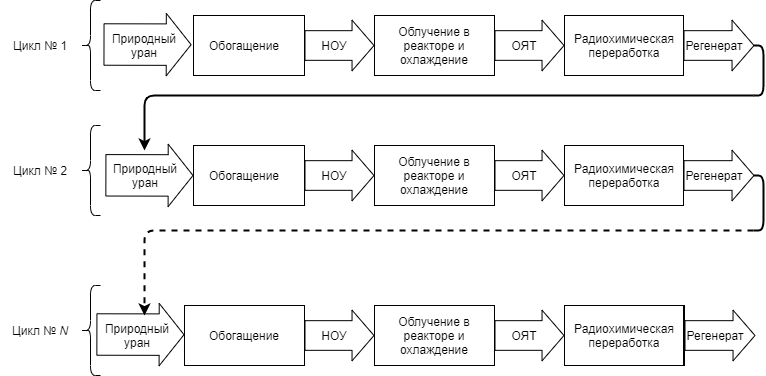
\includegraphics[scale=0.55]{theory/recycling_ru}}
  \caption{Схема многократного рециклирования урана}\label{recycle}
\end{figure}

\begin{figure}[ht]
  \centerfloat{
\includegraphics[scale=1.2]{cascades/ordinary/ordinary}}
  \caption{Схема ординарного трехпоточного каскада. $F$ -- поток питания; $P$ -- поток отбора; $W$ -- поток отвала.}\label{ordinary}
\end{figure}

В соответствии со схемой рис. \ref{recycle} предполагаем, что первичная загрузка реактора осуществлена топливом, изготовленном из обогащенного природного урана. Далее, при обогащении регенерированного урана природный уран используется в качестве материала подпитки, обеспечивающего необходимое количество дополнительного $^{235}$U для изготовления требуемой массы свежего топлива. Далее, процесс рецикла урана с добавлением природного сырья повторяют $N$ раз. Заметим, что материал подпитки необходим в рассматриваемой принципиальной схеме рецикла, так как в реакторе на тепловых нейтронах не достижимо расширенное воспроизводство ядерного топлива, из-за того, что коэффициент воспроизводства делящегося нуклида $^{235}$U в таком типе реакторов меньше единицы \cite{ignatevVliyanieVidaTopliva2020}. 


Как следует из анализа результатов исследований, посвященных вопросам многократного рецикла урана в топливе легководных реакторов, в ходе рециклирования происходит рост (до нескольких раз) концентраций четных изотопов в регенерате после облучения в реакторе \cite{smirnovEvolutionIsotopicComposition2012}. При этом ввиду относительной малости концентрации $^{232}$U на первом (или, в некоторых случаях, на первых двух) рециклах не происходит достижения концентрацией этого изотопа предельных значений в финальном продукте \cite{smirnovApplyingEnrichmentCapacities2018}.
После роста концентраций четных изотопов на первых рециклах, наблюдается их постепенный выход на «плато», начиная с $\approx$3-го рецикла, что обусловлено фиксацией концентрации изотопа $^{232}$U в продукте на уровне $5\cdot10^{-7}$\%, что доказывает возможность многократного рециклирования облученной урановой топливной составляющей.

Таким образом, при анализе вопросов замыкания топливного цикла реакторов на тепловых нейтронах с использованием регенерированного урана необходимо учитывать такие факторы, как общая тенденция к повышению глубины выгорания в современных реакторах, так и рост концентраций четных изотопов в процессе рециклирования урана. Это факторы делают актуальными разработку каскадных обогатительных схем, позволяющих эффективно использовать регенерированный уран при производстве товарного НОУ с учетом всех описанных выше требований и ограничений как в условиях многократного рецикла урана.

Отметим ещё один важный фактор. Очевидно, учитывая, относительно высокую цены переработки ОЯТ наиболее целесообразно максимально вовлекать в повторное использование весь выделенный из него регенерат. Это означает, что если рассматривать отдельный реактор, то логично при получении НОУ из регенерированного урана использовать при его производстве весь выделенный из ОЯТ этого же реактора регенерат. Это будет означать, во-первых, минимизацию потерь $^{235}$U в топливном цикле, и, во-вторых, максимально эффективное использование потенциала ОЯТ для воспроизводства топлива, а, в-третьих, отсутствие нежелательного накопления регенерата на складах. При этом следует сделать акцент на том, что подобное условие не является физическим требованием, а скорее призвано повысить эффективность замыкания топливного цикла реакторов на тепловых нейтронах по урановой составляющей. Схематично это условие иллюстрирует рисунок \ref{reconeto}.

\begin{figure}[ht]
  \centerfloat{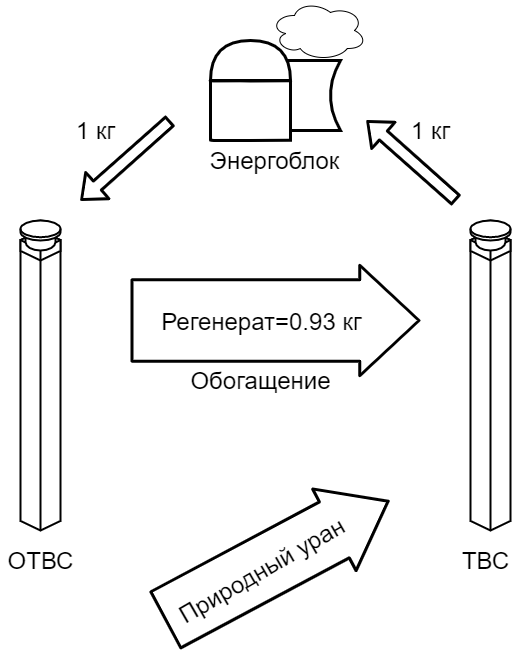
\includegraphics[scale=0.55]{theory/recycling1kg_ru}}
  \caption{Схема замыкания урановой топливной составляющей.}\label{reconeto}
\end{figure}


Учитывая выше сказанное, задача обогащения регенерата в общем случае может быть сформулирована подразумевает: получение заданной массы товарного НОУ требуемого обогащения по $^{235}$U из сырьевого регенерата урана (в том числе многократно рециклированного) с одновременным выполнением ограничений на концентрации четных изотопов, а также при условии расходования всей массы регенерата, выделенного из ОЯТ данного реактора.

Таким образом, с обогащением регенерата урана в каскадах газовых центрифуг связаны определенные сложности, требующие модификации подходов, принятых на разделительных производствах при обогащении природного урана. Все перечисленные факторы сделали актуальными разработки в области поиска оптимальных каскадных схем для обогащения регенерированного урана с учетом требований, предъявляемых к получаемому продукту -- НОУ.

Оптимальность той или иной каскадной схемы зависит от выбранных критериев эффективности. В качестве таких критериев, как правило, используют минимум затрат работы разделения и расхода природного урана для получения единицы товарного НОУ. Эти характеристики в значительной мере определяют величину удельных затрат на получение товарного НОУ.


\section{Промышленный опыт}\label{sec:ch1/sec1}

Возврат урана в топливный цикл по представленной выше схеме опирается на три ключевые технологии:
\begin{enumerate}
  \item Радиохимическую переработку ОЯТ;
  \item Изотопное обогащение регенерированного урана;
  \item Изготовление топлива на основе восстановленного отработавшего топлива.
\end{enumerate}

Что касается первого пункта, в странах, лидирующих в развитии ядерных технологий, с середины прошлого века широко используется технология гидрометаллургической переработки облученного топлива, называемая PUREX \cite{selvaduraySurveyNuclearFuel1979}. В России, технологии связанные с переработкой ОЯТ развиваются особенно успешно благодаря ориентированности отрасли на замыкание ЯТЦ \cite{balihinSostoyaniiPerspektivahRazvitiya2018, efimenkoProblemyPerspektivyRazvitiya2017}. В виду такого стратегического курса отечественной атомной отрасли, запланирован ввод новых мощностей, которые расчитаны на переработку принимаемого ОЯТ из-за рубежа \cite{050519L3942005}. С 2016 г. на <<ФГУП ПО <<МАЯК>> осуществляется переработка партий ОТВС ВВЭР-1000 \cite{PyatyyNacionalnyyDoklad}.

Что касается технологии изотопного обогащения урановых смесей, российская атомная промышленность имеет опыт обогащения регенерированного урана из реакторов ВВЭР-440, который затем использовался в качестве топлива РБМК \cite{VVER10001200Za}. Для этого используют метод прямого обогащения в трехпоточной каскадной схеме. Такая схема реализована для производства исходного сырья для изготовления топлива РБМК на заводе РТ-1 \cite{volkVozvratUranaIz2010}. Этот вариант также апробирован для изготовления опытных тепловыделяющих сборок (ТВС) для реакторов ВВЭР, требующих более высокого уровня обогащения \cite{proselkovAnalizVozmozhnostiIspolzovaniya2003}.
% Здесь важно также отметить, что на сегодняшний день у топливного дивизиона Росатома имеется уникальный технологический задел, связанный с газоцентрифужной технологией, который уже сегодня отражен в доминирующей роли этой технологии на мировом рынке разделительных услуг за счет низкой себестоимости единицы работы разделения, которую обеспечивают энергоэффективные и долговечные разделительные аппараты.

Что касается заключительного пункта, Росатом на одном из заводов фабрикации ядерного топлива осуществлял изготовление опытных образцов тепловыделяющих сборок в том числе на основе зарубежного облученного топлива (из Франции) с повышенным содержанием $^{232}$U \cite{kislovRadiacionnyeAspektyIspolzovaniya}.

Имеющийся в России опыт рециклирования ядерного топлива базируется на смешении регенератов урана, извлекаемых из ОЯТ ВВЭР и ОЯТ транспортных реакторов с высоким содержанием $^{235}$U \cite{international2003iaea}.

При этом зарубежный опыт базируется на однократном использовании MOX-топлива \cite{international2003iaea}.

% При этом, опираясь на передовой уровень разделительной технологии, можно заключить, что задача обогащения регенерата до необходимого для повторного использования в энергетических ядерных реакторах уровня концентрации изотопа $^{235}$U может быть решена.

Таким образом, сложившаяся к текущему моменту в России научно-производственная база с наращиваемыми объемами промышленных разделительных мощностей, основанных на центробежном методе разделения, является основным аргументом в пользу готовности к вовлечению регенерата в топливный цикл легководных реакторов.

Однако, для практической реализации долгосрочных планов отрасли по замыканию ЯТЦ и расширению предложения международных топливных поставок, что предусматривает многократное рециклирование делящихся материалов, необходимо решить задачу возврата регенерата в ЯТЦ, подразумевая наличие вышеизложенных ограничений \cite{RosatomGoskorporaciyaRosatoma,panteleyOsobennostiMezhdunarodnogoSotrudnichestva2017}.

Для анализа возможности решения задачи рецикла урана в рамках поставленных ограничений с помощью ранее предложенных схем, перейдем к их подробному рассмотрению.

\section{Обзор способов обогащения регенерата урана в каскадах центрифуг}

Ниже приведены результаты критического анализа каждой из схем, позволяющие сделать вывод как об их достоинствах и недостатках, так и о возможности их использования для решения задачи многократного рецикла урана в топливе современных реакторов на тепловых нейтронах.

Принимая во внимание сложность сформулированной выше задачи обогащения регенерата по отношению к случаю обогащения природного урана, непосредственное применение штатной схемы обогащения -- ординарного или трехпоточного каскада (рисунок 1) имеет существенные ограничения и в общем случае поставленную задачу не решает. Главная причина состоит в том, что подобный каскад имеет всего один выходящий поток отбора, в котором, одновременно будут концентрироваться, как целевой  $^{235}$U, так и четные изотопы. В результате ординарный каскад позволяет лишь обогащать относительно «чистые» составы регенерата, в которых исходные содержания четных изотопов меньше (на порядок или более), чем их допустимые пределы в товарном НОУ. Однако эти условия, очевидно, невыполнимы при многократном рецикле урана.
Проведенные сравнительный анализ предложенных способов обогащения регенерата позволяет условно разделить их на 3 типа: схемы с разбавлением четных изотопов,  схемы с отделением четных изотопов, «гибридные» схемы. 
Ниже проанализированы каскадные схемы каждого из указанных типов. В Приложении представлены результаты тестовых расчётов обогащения регенерата различного исходного состава для большинства рассмотренных ниже схем с целью оценки их эффективности для решения поставленной задачи.

\subsection{Каскадные схемы с разбавлением четных изотопов}

Ряд из предложенных каскадных схем обогащения регенерата в качестве основного фактора, корректирующего изотопный состав регенерата в процессе его обогащения, используют разбавление четных изотопов урановой смесью, которая их не содержит. В качестве таких разбавителей чаще всего рассматривают природный уран, однако это могут быть также обедненный или низкообогащенный уран.

Простейшие схемы с разбавлением основаны на использовании штатного ординарного каскада. Рассмотрим такие схемы, которые могут быть реализованы следующими способами (рис. \ref{fig:diagram1}) \cite{sulaberidzeNekotoryhRazdelitelnyhProblemah2004,smirnovKaskadnyeShemyZadachah2012}:

\begin{enumerate}
  \item Смешивание регенерированного урана и природного (или обедненного) урана перед подачей в каскад рис. (рис. \ref{fig:diagram1}.1).
  \item Получение обогащенной фракции из регенерата и последующее ее разбавление природной урановой смесью (рис. \ref{fig:diagram1}.2).
  \item Получение НОУ из природного урана путем его прямого обогащения, с последующим разбавлением регенератом (рис. \ref{fig:diagram1}.3).
\end{enumerate}

\begin{figure}[ht]
  \centerfloat{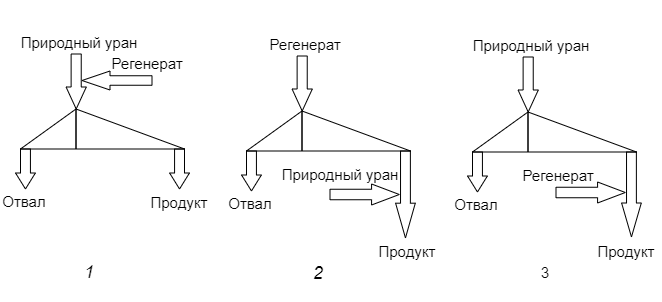
\includegraphics[scale=0.7]{cascades/diagram1}}
  \caption{Схемы на основе ординарного каскада}\label{fig:diagram1}
\end{figure}

Для всех вариантов схем рис. \ref{fig:diagram1} сотношение между расходом регенерата и разбавителем природного происхождения определяется пределом допустимой концентрации $^{232}$U в конечном продукте -- низкообогащенном уране. Также компенсируется отрицательная реактивность $^{236}$U с помощью добавочной концентрации $^{235}$U к той, что требуется для НОУ-топлива с заданными свойствами.

Основным преимуществом таких схем является простота реализации, поскольку нет необходимости в модификации самого каскада, так как операции разбавления осуществляются за его пределами.

В качестве недостатков таких схем можно выделить:
\begin{enumerate}
  \item отсутствие возможности очищать регенерированный уран от четных изотопов, так как такие схемы основаны исключительно на разбавлении четных изотопов до допустимых концентраций;
  \item потери работы разделения, возникающие из-за смешения потоков с различными изотопными концентрациями $^{235}$U;
  \item невозможность выполнения условия «полного использования регенерированного урана» при многократном рецикле \cite{smirnovApplyingEnrichmentCapacities2018} (см. Приложение/глава 3);
  \item выполнение ограничений по концентрации $^{232}$U в продукте напрямую зависит от концентрации указанного изотопа в поступившем в обогащение регенерате;
  \item для схем рис. \ref{fig:diagram1}.1--\ref{fig:diagram1}.2 имеет место загрязнение 100\% задействованных в обогащении регенерированного урана разделительных мощностей, что делает проблематичным их дальнейшее «перепрофилирование» на обогащение природного урана, по крайней мере в случае длительной (в течение нескольких лет) работы с регенерированным ураном.
\end{enumerate}

Подытоживая рассмотрение простейших разбавляющих схем обогащения регенерата можно отметить, что их использование не позволяет оцищать регенерат от чётных изотопов, вся масса которых фактически полностью переносится в отбор каскада, что затрудняет использование таких схем в условиях многократного рецикла, когда концентрации чётных изотопов возрастают. Поэтому такие каскадные схемы потенциально применимы только для обогащения относительно «чистого» состава регенерата, в котором содержание $^{232}$U меньше допустимой нормы на порядок и более, что нехарактерно для изотопных составов выгружаемого из активной зоны современных ВВЭР облученного топлива при многократном рецикле урана \cite{bormanTehnikoekonomicheskiyAnalizVozmozhnyh2012}. 

Другие варианты каскадных схем с разбавлением чётных изотопов основаны на использовании так называемых многопоточных каскадов \cite{sulaberidzeQuasiidealCascadesAdditional2006}. В отличие от предыдущих вариантов в рассматриваемом случае разбавление регенерата осуществляют непосредственно в каскаде путем подачи одного или нескольких разбавителей в качестве дополнительного питания каскада параллельно с самим регенерированным ураном. Подобное разбавление одним или несколькими разбавителями можно осуществить в каскадах с двумя или тремя внешними питаниями (рисунки 3, 4).


\subsection{Каскады с дополнительными внешними потоками (многопоточные схемы)}

Проанализируем многопоточные каскады, начиная с самых простых схем такого рода.

Существуют многопоточные модификации каскадных схем для обогащения регенерированного урана, также основанные на использовании эффекта разбавления регенерата смесями, не содержащими четных изотопов $^{232,236}$U. Такие схемы представляют из себя одиночные каскады с дополнительными входящими или исходящими потоками.

При подаче дополнительного питания в каскад для минимизации смешивания концентраций $^{235}$U и, соответственно уменьшения потерь работы разделения, дополнительные потоки питания ступени, подобранные таким образом, чтобы концентрация целевого компонента в питающем потоке была как можно ближе к концентрации в принимающей ступени. 

В \cite{sulaberidzeQuasiidealCascadesAdditional2006} предожена схема с двумя потоками питания: природный уран и регенерат (рис. \ref{fig:2_inputs}).
\begin{figure}[ht]
  \centerfloat{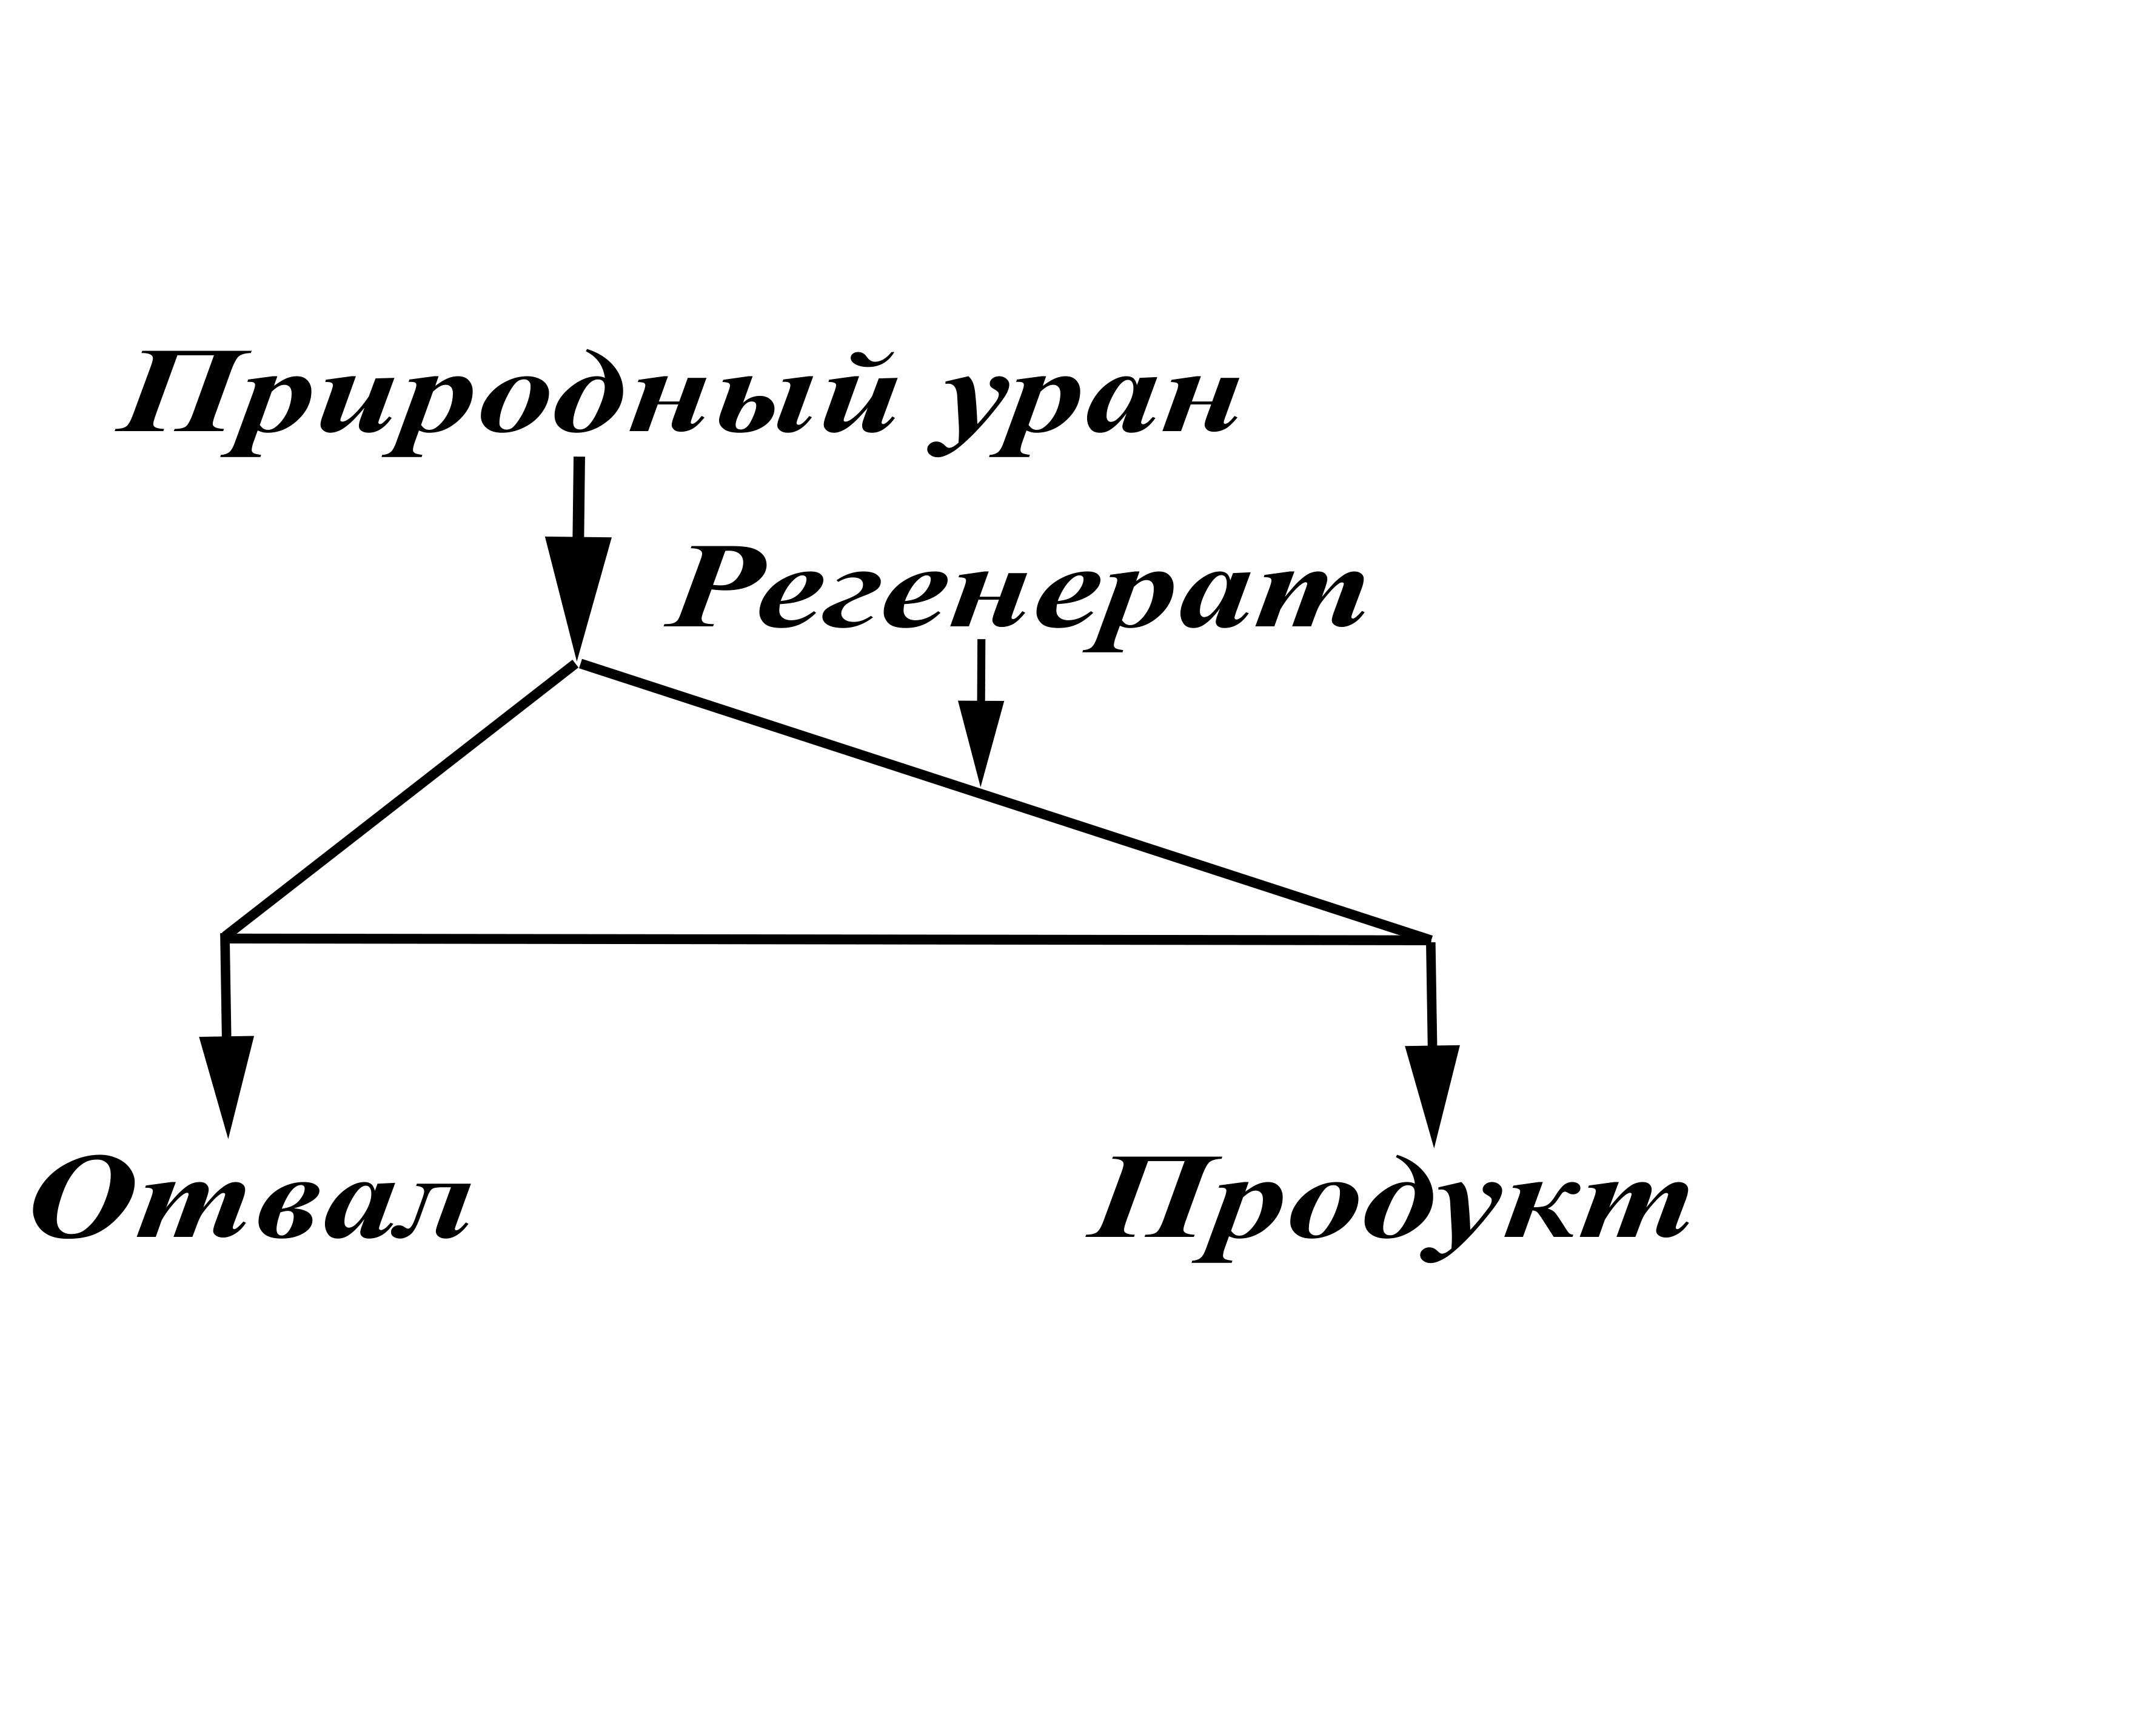
\includegraphics[scale=0.07]{cascades/2in}}
  \caption{Каскад с дополнительным потоком питания}\label{fig:2_inputs}
\end{figure}

Принципиально такую схему можно рассматривать как усовершенствование схемы обогащения в ординарном каскаде предварительно смешанных природного (или обедненного) и регенерированного урана (рис. \ref{fig:diagram1}.1). Такая модификация обладает по сравнению с трехпоточным каскадом преимуществом по двум причинам:

Во-первых, метод введения дополнительного потока в отличную от основного потока питания ступень каскада позволяет избежать потери работы разделения в ходе смешения потоков с различными концентрациями $^{235}$U, располагая дополнительный входной поток там, где концентрации внешнего и внутреннего потоков в $^{235}$U совпадают \cite{smirnovKaskadnyeShemyZadachah2012, sulaberidzeQuasiidealCascadesAdditional2006}.

Во-вторых, в схеме с дополнительным потоком питания регенерат, ввиду содержания в нем $^{235}$U на уровне выше, чем в природном уране (и тем более выше, чем в обедненном уране как альтернативе природному в качестве разбавителя регенерата), подается в ступень расположенную ближе к отбору каскада, а значит самый легкий изотоп $^{232}$U обогащается в меньшей степени за счет того, что проходит через меньшее число последовательных ступеней.
% Тем не менее, при повторном использовании регенерированного урана из топлива ВВЭР, даже такой подход может обеспечить значительную экономию природного урана ($\approx$16\% согласно \cite{alekseevPossibleScenariosTransition2020}).
% Суммарная же экономия природного урана за всю серию рециклов будет складываться из уменьшающихся с каждым рециклом показателей сэкономленного природного сырья \cite{colemanEvaluationMultipleSelfrecycling2010,smirnovEvolutionIsotopicComposition2012}).

Однако добавочный поток питания представляет собой, в сущности, «разбавление» четных изотопов  $^{232,234}$U, содержащихся в регенерате, что также как и для схемы ординарного каскада связано с невозможностью обеспечить условие полного возврата ОЯТ в ЯТЦ, то есть использования 1 кг ОЯТ на 1 кг НОУ продукта в условиях многократного рецикла. 
% Это условие необходимо для полного замыкания цикла по урану и, тем самым, корректного контроля за оборотом делящихся материалов при экспортных поставках топлива. С другой стороны, в условиях российской ядерной энергетики оно позволяет не создавать складской запас регенерированного урана, хранение которого требует определенных затрат.

% Выполнение такого условия достижимо только для изотопных составов первого (иногда второго) рецикла топлива легководного реактора.
% Таким образом, с помощью такой схемы нельзя обеспечить заданную пропорцию вовлечения регенерированного урана в условиях многократного рецикла, так как, начиная с третьего цикла, расходовать требуемый уровень регенерата становится невозможно из-за ухудшения изотопного состава урана и наличия ограничений на изотопы $^{232,236}$U \cite{smirnovApplyingEnrichmentCapacities2018}.


% Для отечественной ядерной индустрии, $^{235}$U из <<богатых>> источников ОГФУ ($\approx$0.3\%), является важным источником сырья для производства ядерного топлива, а также доходным международным бизнесом \cite{oecdManagementDepletedUranium2001}.
% Имеющиеся в мире запасы $\approx$1.2 миллиона тонн <<богатых>> хвостов (0.3\%) дают эквивалент 336 тысяч т. эквивалента природного урана при концентрации $^{235}$U в отвале 0.14\%. Этого достаточно, чтобы обеспечить на 5 лет топливом весь мировой парк энергетических реакторов.
% Стоит отметить, что наличие ОГФУ такой категории связано с историей развития обогатительного производства. Ввиду того, что диффузионный метод разделения -- технология первого поколения -- требует колоссальных затрат энергии на единицу РР, получение обогащенного продукта было целесообразней осуществлять с б'ольшими затратами природного урана.
% Напомним, что выбор в пользу затрат на каждый из этих показателей связан с компромиссом, определяемым, во многом, экономическими факторами: себестоимостью единицы работы разделения и стоимостью сырья. 
% Итак, согласно годовому отчету ГК <<Росатом>> 2019 г. (стр. 45 \cite{ITOGIDEYaTELNOSTIGOSUDARSTVENNOY}), поставки из вторичных источников (складские запасы энергокомпаний и некоторых государств, дообогащение обедненного гексафторида урана, регенерированный уран и пр.) оцениваются на уровне 20 тыс. т в эквиваленте природного урана.

% Так, в \cite{smirnovApplyingEnrichmentCapacities2018} были рассчитаны основные показатели, характеризующие экономику производства обогащенного урана: расход природного урана и затраты работы разделения (РР).

Используя схему с дополнительным потоком питания (рис. \ref{fig:2_inputs}) на первых двух рециклах урана в топливе легководных реакторов можно достичь экономии природного урана на уровне $\approx$20\% \cite{smirnovApplyingEnrichmentCapacities2018}. Затем, этот показатель ухудшается, так как при заданных условиях, к третьему циклу повторного использования происходит значительное ухудшение изотопного состава, заключающееся в накоплении в урановой фракции нежелательных четных изотопов $^{232,234,236}$U, так называемая <<деградация>> изотопного состава.

% Отсюда вытекает интерес к исследованию возможности повышения предела экономии природного урана. Для этого необходимо искать альтернативный разбавитель. Например, таким материалом может послужить обедненный уран (так называемые «хвосты» (или отвалы) -- побочный продукт процесса обогащения), который благодаря современным разделительным технологиям стало возможно использовать как ресурс делящегося $^{235}$U \cite{oecdManagementDepletedUranium2001, ITOGIDEYaTELNOSTIGOSUDARSTVENNOY}. При этом использование такого разбавителя может иметь место не только в качестве прямой альтернативы природному урану, но и в качестве дополнительного потока питания, что позволит добиться умеренного увеличения затрачиваемой работы разделения, по сравнению с отказом от использования природного урана и заменой его на ОГФУ. Перейдем к описанию такой схемы каскада, позволяющей задействовать ОГФУ в повторном обогащении регенерированного урана.

Развитием этой схемы стала схема с тремя потоками питания изображена на рис. \ref{fig:3_inputs}, где $F_{1}, F_{2}, F_{3}$ -- потоки питания в виде ОГФУ, природного урана и регенерата, соответственно; а $W$ и $P$ -- потоки отвала и питания. Дополнительные входные потоки в этой схеме располагают таким образом, чтобы минимизировать смешивание, происходящее из-за разности концентраций изотопа $^{235}$U в подаваемой в каскад изотопной смеси и в ступени каскада, в которую подается питающая смесь. Подробное описание математической модели приведено в \cite{smirnovEnrichmentRegeneratedUranium2014}. Такая схема может быть реализована и таким образом, чтобы вместо природного урана разбавителем выступал низкообогащенный уран, предварительно произведенный из природного урана, имеющий уровень обогащения 1,0-2,0\% \cite{smirnovDilutionRecycledUranium2015}. 

\begin{figure}[ht]
  \centerfloat{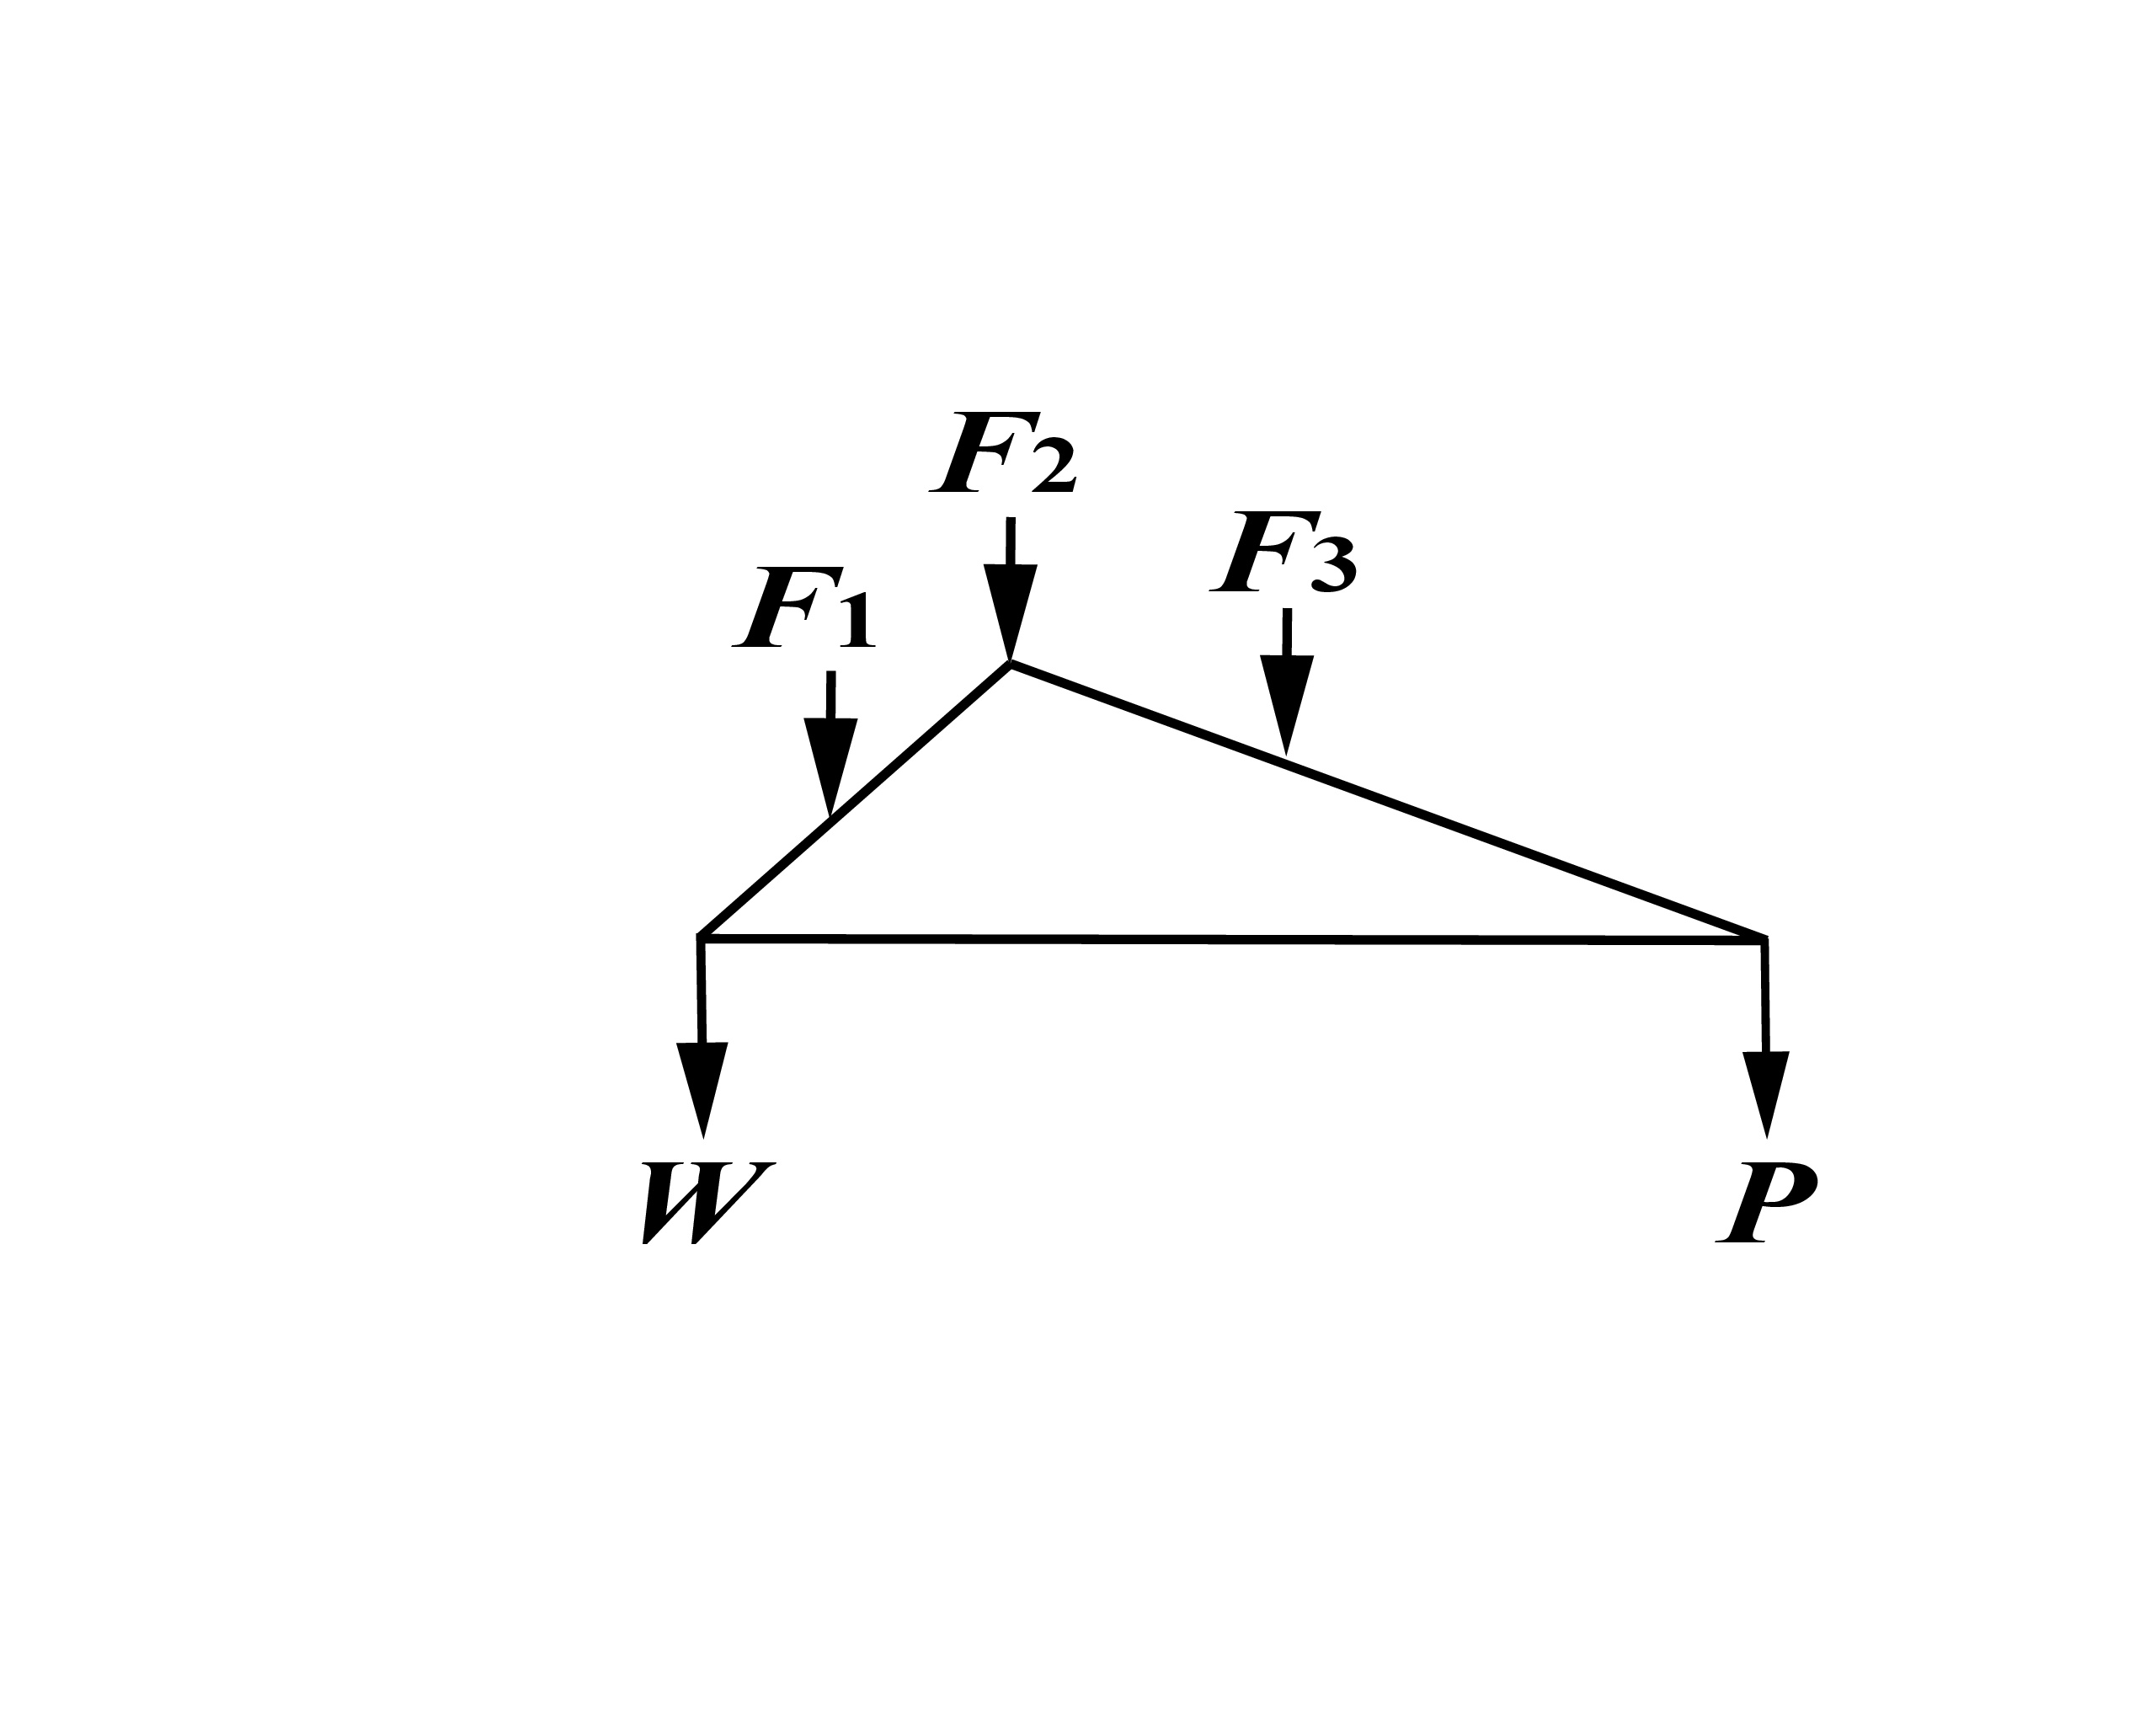
\includegraphics[scale=0.17]{cascades/3in}}
  \caption{Каскад с тремя потоками питания}\label{fig:3_inputs}
\end{figure}

% \begin{figure}[ht]
%   \centerfloat{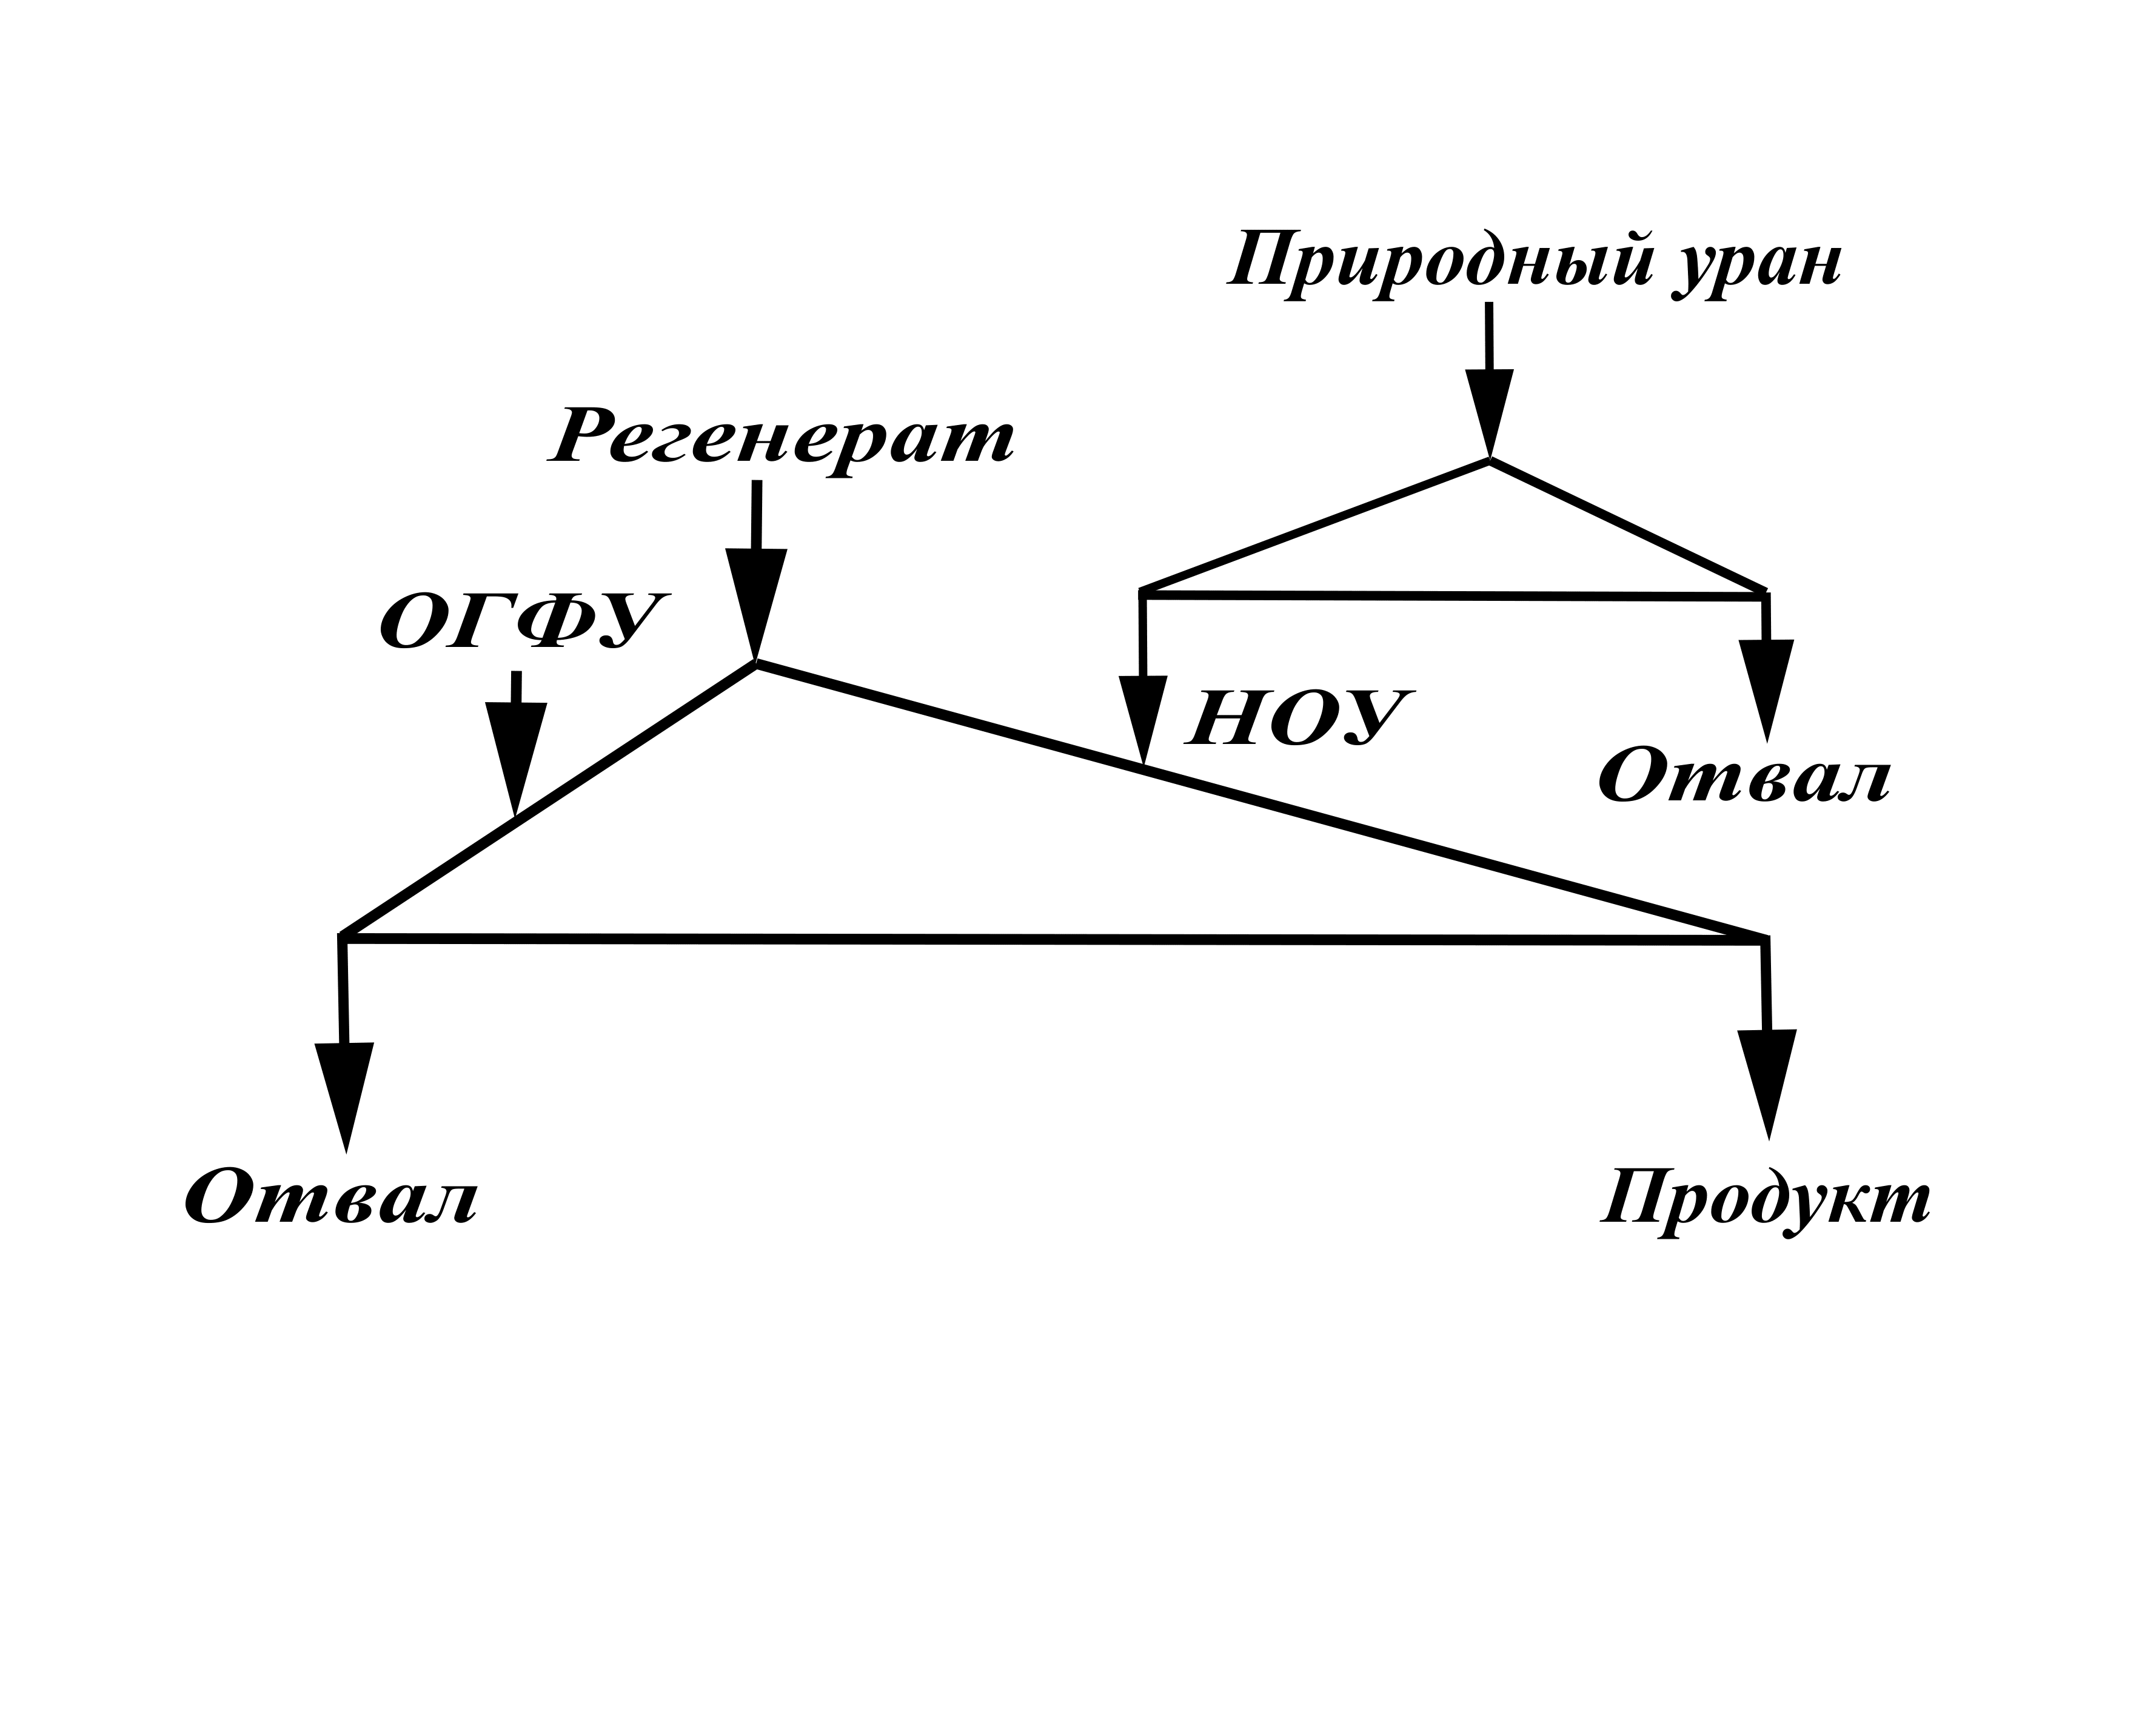
\includegraphics[scale=0.1]{cascades/double_3feeds}}
%   \caption{Двойной каскад, использующий каскад с тремя питаниями}\label{fig:double_3feeds}
% \end{figure}

% Использование в качестве дополнительного потока питания каскада с тремя питаниями потока НОУ, вместо потока природного урана, позволяет улучшить желаемые показатели экономии природного урана и затрат работы разделения за счет возможности использования обогатительной части каскада меньшей длины, необходимой для достижения в отборной части необходимого уровня обогащения по $^{235}$U, что достигается за счет подачи в каскад потока с большим содержанием изотопа $^{235}$U. В итоге, концентрация изотопа $^{232}$U повышается в меньшей степени, за счет прохождения потоком регенерата меньшего количества последовательных ступеней. Эта схема получила дальнейшее развитие в \cite{smirnovEvaluatingEffectivenessDilution2016}, где было продемонстрирована возможность снизить с помощью нее себестоимость производства товарного НОУ-продукта. Однако, схемы на основе каскада с тремя питаниями (с двумя дополнительными потоками питания) не позволяют добиться выполнения условий полного возврата регенерата в цикл и, как и ранее рассмотренные схемы с дополнительными потоками питания, обеспечивают возможность вовлечения регенерата в топливный цикл преимущественно за счет его разбавления смесями, не содержащими $^{232}$U \cite{smirnovApplyingEnrichmentCapacities2018}.

Преимущества схемы с тремя питаниями (рис. \ref{fig:3_inputs}) заключается в следующих ее свойствах:

\begin{enumerate}
  \item приобретается возможность настраивать каскад для достижения желаемого баланса между показателями затрат природного урана и работы разделения, то есть варьировать интегральные характеристики разделительного процесса, отражающие его экономику. Снижение расхода природного урана потребует повышения затрачиваемой работы разделения и наоборот. Такой подход может позволить добиться оптимума удельных затрат при производстве НОУ-продукта. В качестве примера реализации желаемых производственных показателей, можно получить экономию половины природного урана на каждом рецикле, по сравнению с ординарным каскадом для обогащения природного урана   \cite{smirnovApplyingEnrichmentCapacities2018}. Для этого на каждом рецикле при производстве товарного НОУ с помощью такой схемы необходимо будет затрачивать на $\approx$50--60\% больше работы разделения, по сравнению с ординарным каскадом для обогащения природного урана, получающим продукт с эквивалентной эффективной концентрацией $^{235}$U;
  \item частичное решение проблемы утилизации накопленных объемов обедненного урана \cite{smirnovEnrichmentRegeneratedUranium2014}. Поскольку гексафторид урана является агрессивным веществом, его хранение связано с затратами, и емкости для хранения следует время от времени заменять из-за коррозионных процессов \cite{fitchOPTIONSDISPOSALREAPPLICATION2009, oecdManagementDepletedUranium2001}.
\end{enumerate}

Следует отметить, что этот подход предполагает снижение содержания $^{235}$U в образовавшемся ОГФУ, по сравнению с исходным, и требует исследования перспектив дальнейшего использования такого материала в бланкетах реакторах-бридерах \cite{smirnovApplyingEnrichmentCapacities2018}.
Произведенный посредством схемы рис. \ref{fig:3_inputs} ОГФУ, содержащий минорные изотопы, подлежит переводу в стабильную форму с помощью установок дефторирования типа «W-ЭХЗ» \cite{RosatomGoskorporaciyaRosatoma}. Такая переработка, заключается в обеcфторивании и переводе в более устойчивое химическое соединение -- закись-окись урана  \cite{PererabotkaOGFUObrazovaniem2014}.
% <<дважды обедненный>> 

Таким образом, схемы с дополнительными питаниями (рис. \ref{fig:2_inputs} и рис. \ref{fig:3_inputs}) не способны обеспечить выполнение условия задействования всего объема регенерата в процессе рециклирования урана в качестве топлива ВВЭР в условиях многократного рецикла. Это обстоятельство имеет место начиная со второго или третьего рецикла в зависимости от заданной величины допустимой концентрации $^{235}$U в товарном НОУ ($2\cdot10^{-7}$\% или $5\cdot10^{-7}$\%) \cite{smirnovEvolutionIsotopicComposition2012}. Основная причина состоит в том, что данная схема, как и все предыдущие варианты имеет лишь один выводной поток, обогащенный по легким компонентам. В этом потоке неминуемо одновременно с целевым изотопом  $^{235}$U концентрируются и все нежелательные четные изотопы $^{232,234,236}$U. Таким образом, комбинирование разбавителей лишь дает возможность варьировать расходные характеристики схемы, но не корректировать изотопный состав получаемого продукта. То есть в конечном счете все вариации данной схемы являются лишь разбавляющими схемами, как и простейшие модификации ординарного трехпоточного каскада (рис. \ref{fig:diagram1}.1--\ref{fig:diagram1}.3).

% Итак, исходя из результатов работы \cite{smirnovApplyingEnrichmentCapacities2018}, схема (рис. \ref{fig:3_inputs}), как и схема рис. \ref{fig:2_inputs}, для заданных составов, характерных современным ВВЭР, позволяет обеспечить полный возврат урана в ядерный топливный цикл только для двух первых рециклов урановой компоненты из-за быстрого накопления четных изотопов  $^{232,234,236}$U, от которых в такой схеме невозможно произвести очистку, выводя легкие изотопы из системы $^{232,234}$U.

% Важность сдерживания накопления $^{232}$U при многократном переиспользовании была показана в работе \cite{smirnovEvolutionIsotopicComposition2012}. Введение ограничения на $^{232}$U позволяет замедлить рост концентрации $^{236}$U в изотопном составе рециклируемого топлива, что позволяет при производстве свежего НОУ затрачивать меньше $^{235}$U на компенсацию нейтронного поглотителя $^{236}$U в виде дополнительной добавки делящегося изотопа.

% Анализ перечисленных выше работ позволяет поставить проблему очистки изотопных составов от четных изотопов, которые имеют тенденцию накапливаться от рецикла к рециклу, приводя к ухудшению изотопного состава за счет накопления в нем изотопов $^{232,234,236}$U.

% Однако, как было отмечено, во всех рассмотренных схемах заметное снижение содержания изотопов $^{232,234,236}$U в финальном НОУ достигается, прежде всего, за счет разбавления регенерата внутри каскада смесями, полученными из урана природного состава (НОУ, ОГФУ).

% Отсюда возникает вопрос очистки изотопного состава рециклируемого материала от четных $^{232,234,236}$U, чтобы сдержать их накопление от рецикла к рециклу.

% В качестве дополнительного аргумента для поиска альтернативных каскадов, позволяющих выводить из системы $^{232,234,236}$U, приведем следующий факт.
% В последнее время конструкция ВВЭР развивалась к увеличению максимального выгорания топлива (до 70 $\frac{МВт*сут.}{кг}$ U в ВВЭР-1200) \cite{asmolovNewGenerationFirstofthe2017}, с целью снижения стоимости топливной составляющей \cite{andrianovaPovyshenieVygoraniyaTopliva2008}.
% А так как, согласно природе цепной реакции, рост остаточного содержания $^{232,234,236}$U пропорционален уровню выгорания \cite{VeryHighBurnups2006}, схемы, нацеленные на очистку $^{232,234,236}$U представляются в будущем более перспективными.

% К тому же, в случае успеха в продвижении российских услуг по реконверсии RepU на мировом рынке, очистка от $^{232}$U может быть востребована в силу ограничения лицензии российского оператора ($5\cdot10^{-7}$\% (5ppb) по $^{232}$U), если не будут применены иные способы улучшения изотопного состава.
% Однако существуют практики возврата регенерата в ЯТЦ, для которых проблема очистки регенерата от четных $^{232,234}$U не актуальна вне необходимости многократного рецикла. Так, Французская электроэнергетическая компания EDF выбрала стратегию прямого обогащения регенерированного урана. Такой подход воплощен на АЭС Cruas, которая имеет лицензию на работу с топливом, в котором ограничение содержания $^{232}$U в 6 раз выше ограничения, принятого в РФ, и составляет 30 ppb.


% Перейдем к исследованию способов вовлечения регенерата урана в производство НОУ, связанные не только с разбавлением регенерата не содержащими искусственных четных изотопов смесями. Такие способы предлагают идею частичного удаления нежелательных изотопов из каскада. Некоторые варианты схем, опирающиеся на эту идею, основаны на включении дополнительного отбора вещества на одной из ступеней каскада.

\subsubsection{Каскад с дополнительным потоком отбора}

Каскад с промежуточным отбором продукта был предложен для возможности осуществлять частичную «очистку» исходного регенерата от четных изотопов $^{232,234,236}$U параллельно с производством основного НОУ-продукта (рис. \ref{fig:3_out}) \cite{zhurinSPOSOBPERERABOTKIZAGRYaZNENNOGO, palkinAnaliticheskiyRaschetSoderzhaniya2007}. В качестве материалов, которые необходимо очистить от изотопов $^{232,234,236}$U посредством такой схемы, помимо регенерированного урана, также можно рассматривать составы загрязненного урана природного состава, а также «хвостов» процесса обогащения \cite{palkinSeparationUraniumIsotopes2010}. Посредством реализации схемы рис. \ref{fig:3_out}, использующей в качестве потока разбавителя природный уран, а в качестве основного -- регенерат, в потоке основного продукта получают НОУ требуемых характеристик, а в качестве промежуточного продукта получают состав урана с пониженным содержанием четных изотопов \cite{palkinSeparationUraniumIsotopes2010}.
\begin{figure}[ht]
  \centerfloat{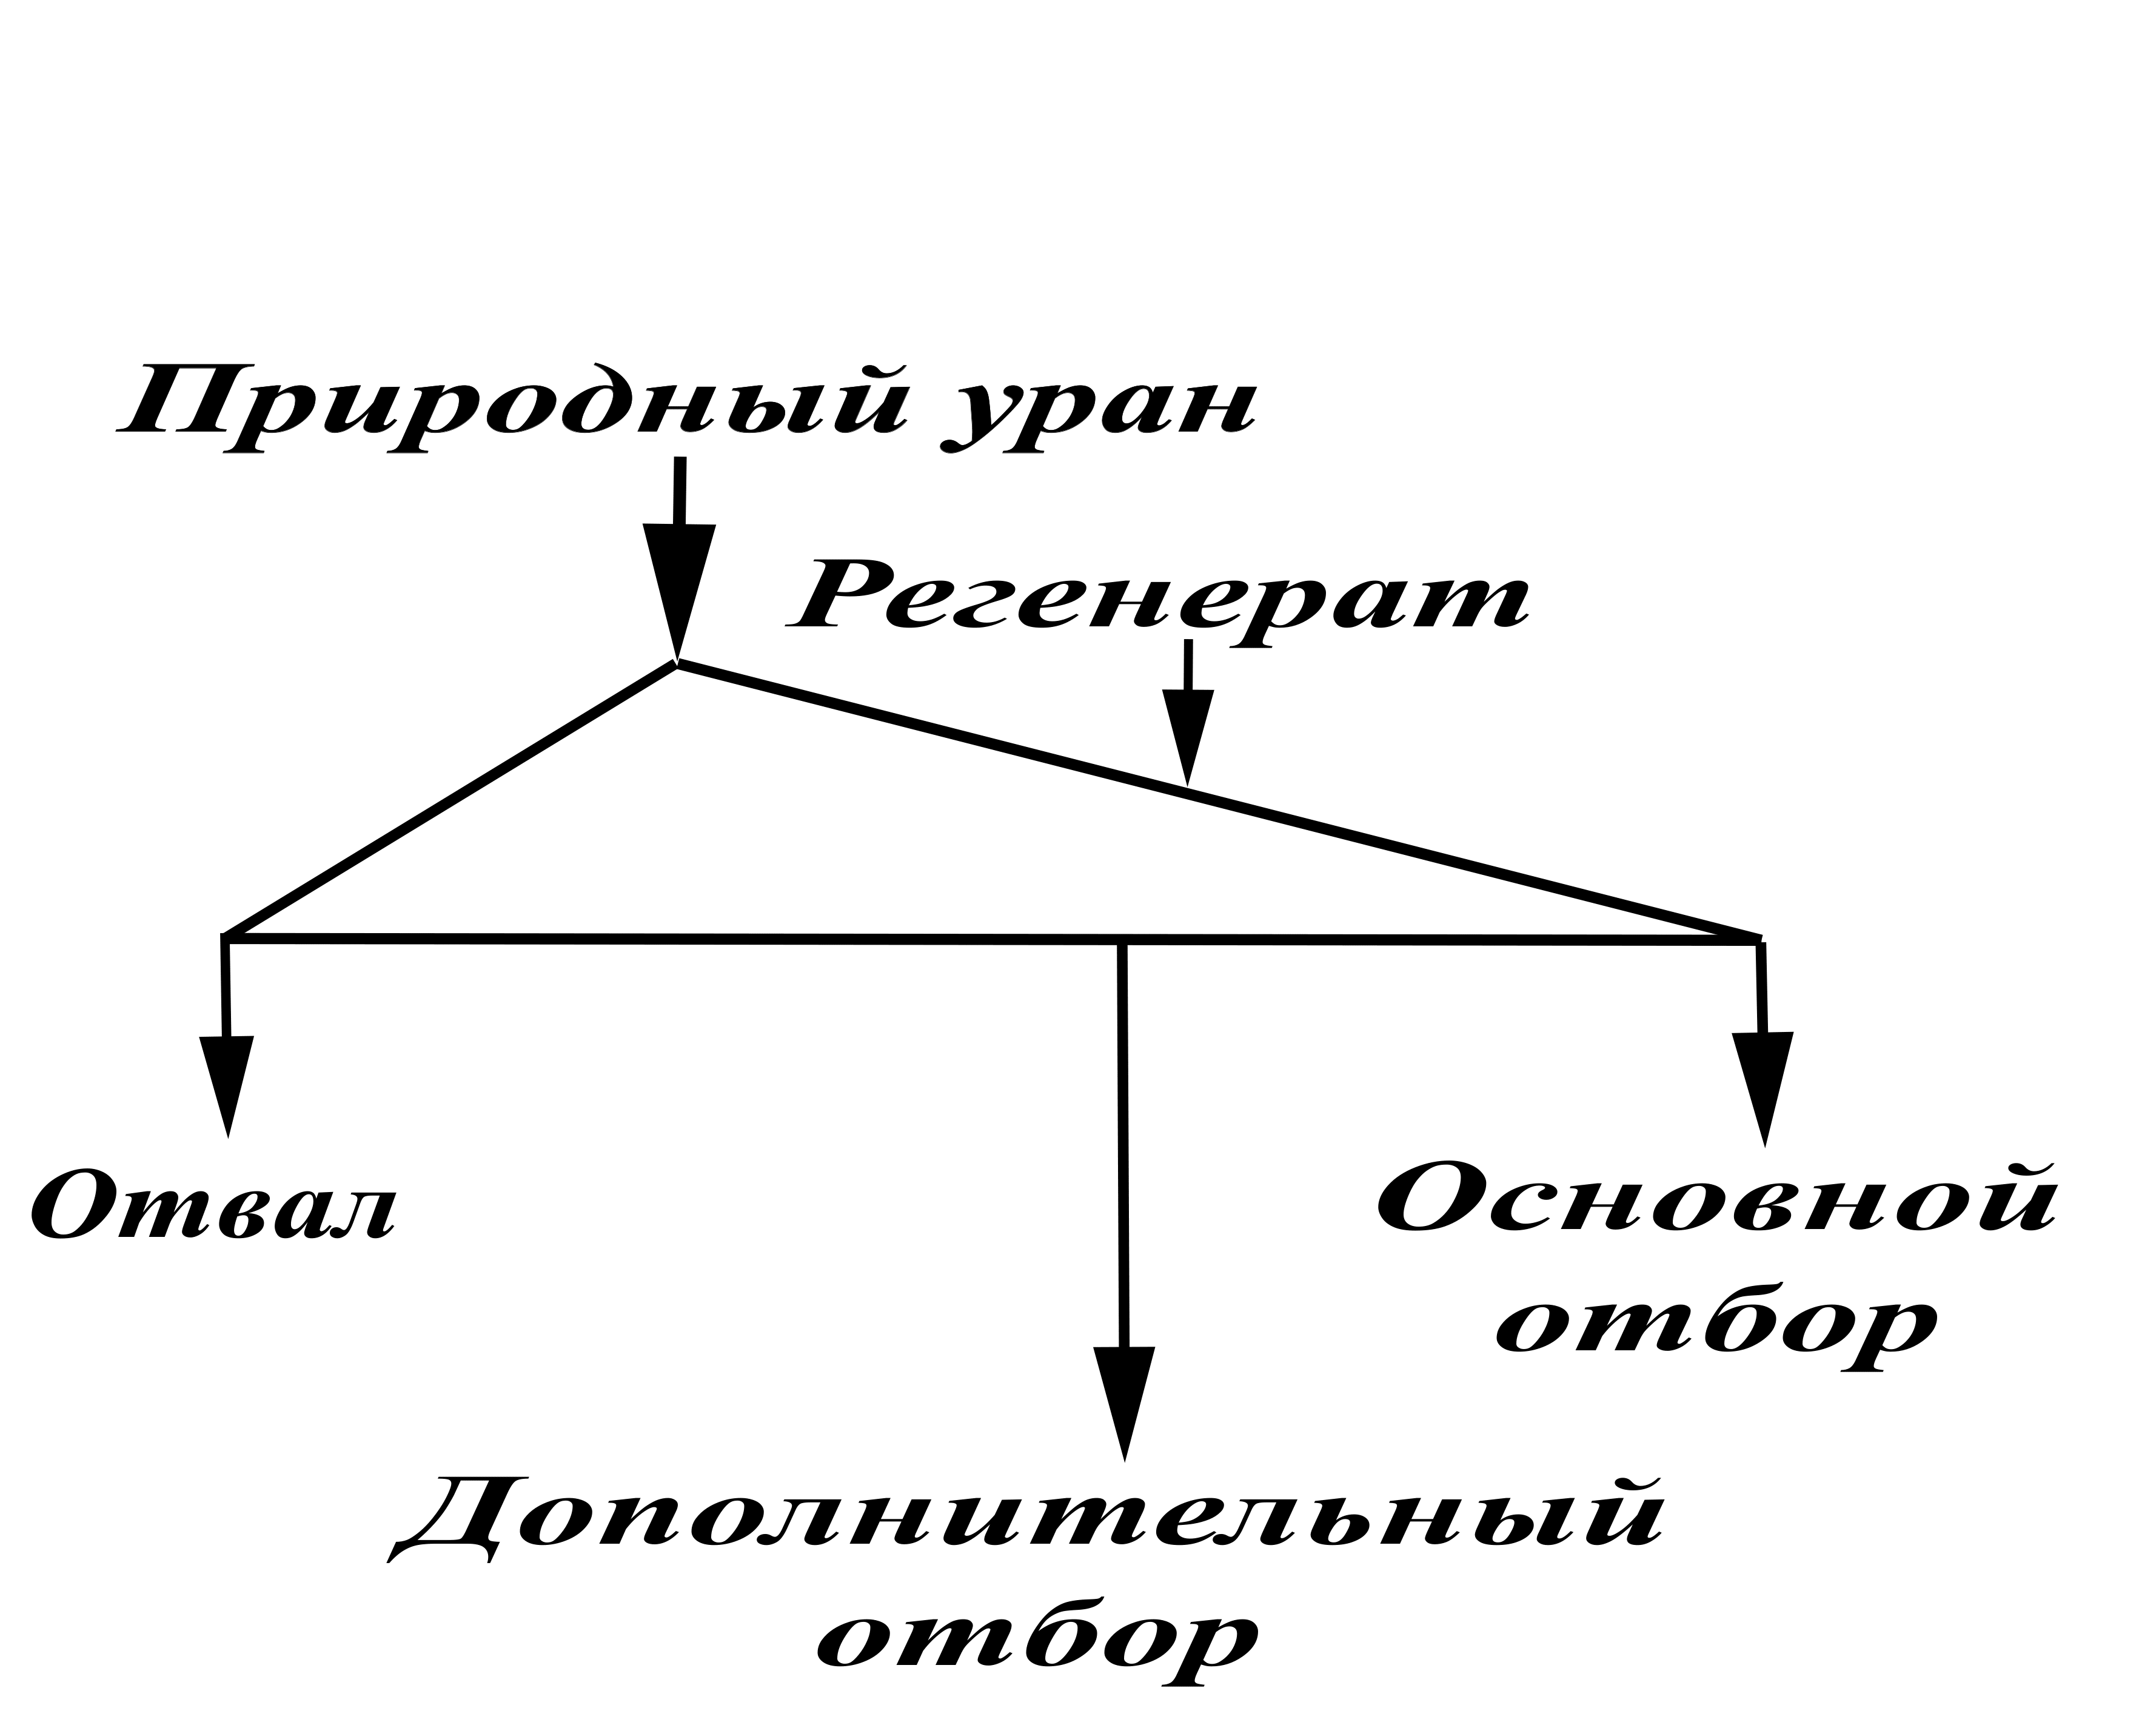
\includegraphics[scale=0.07]{cascades/3out}}
  \caption{Каскад с дополнительным потоком отбора для очистки регенерированного урана от минорных изотопов}\label{fig:3_out}
\end{figure}

В отборе рассматриваемой каскадной схеме должен производиться продукт заданной концентрации изотопа $^{235}$U, а в промежуточном отборе -- полупродукт с уменьшенным содержанием минорных изотопов и концентрацией $^{235}$U близкой к соответствующей величине в поступившем на обогащение регенерате.

% Получение в выходящем потоке дополнительного отбора смеси с пониженными концентрациями $^{232,234,236}$U и схожей с исходным питающим потоком регенерата концентрацией $^{235}$U, позволяет более эффективно использовать такой полупродукт для производства товарного НОУ \cite{palkinSeparationUraniumIsotopes2010}. Концентрация $^{235}$U в этом <<очищенном>> продукте подбирается так, чтобы она минимально отличалась от концентрации в потоке дополнительного питания в виде регенерата. Это позволяет при соблюдении эквивалентности этих потоков исключить потери работы разделения. В результате такой очистки исходного регенерата содержание всех четных изотопов значительно снижается. Низкообогащенный уран с концентрациями $^{232,234,236}$U, удовлетворяющими требования ASTM для коммерческого продукта, может быть получен из такого подготовленного промежуточного продукта путем его прямого обогащения как изображено на рис. \ref{fig:int_double} \cite{shopenSposobPolucheniyaRazbavitelya2008}.

% \begin{figure}[ht]
%   \centerfloat{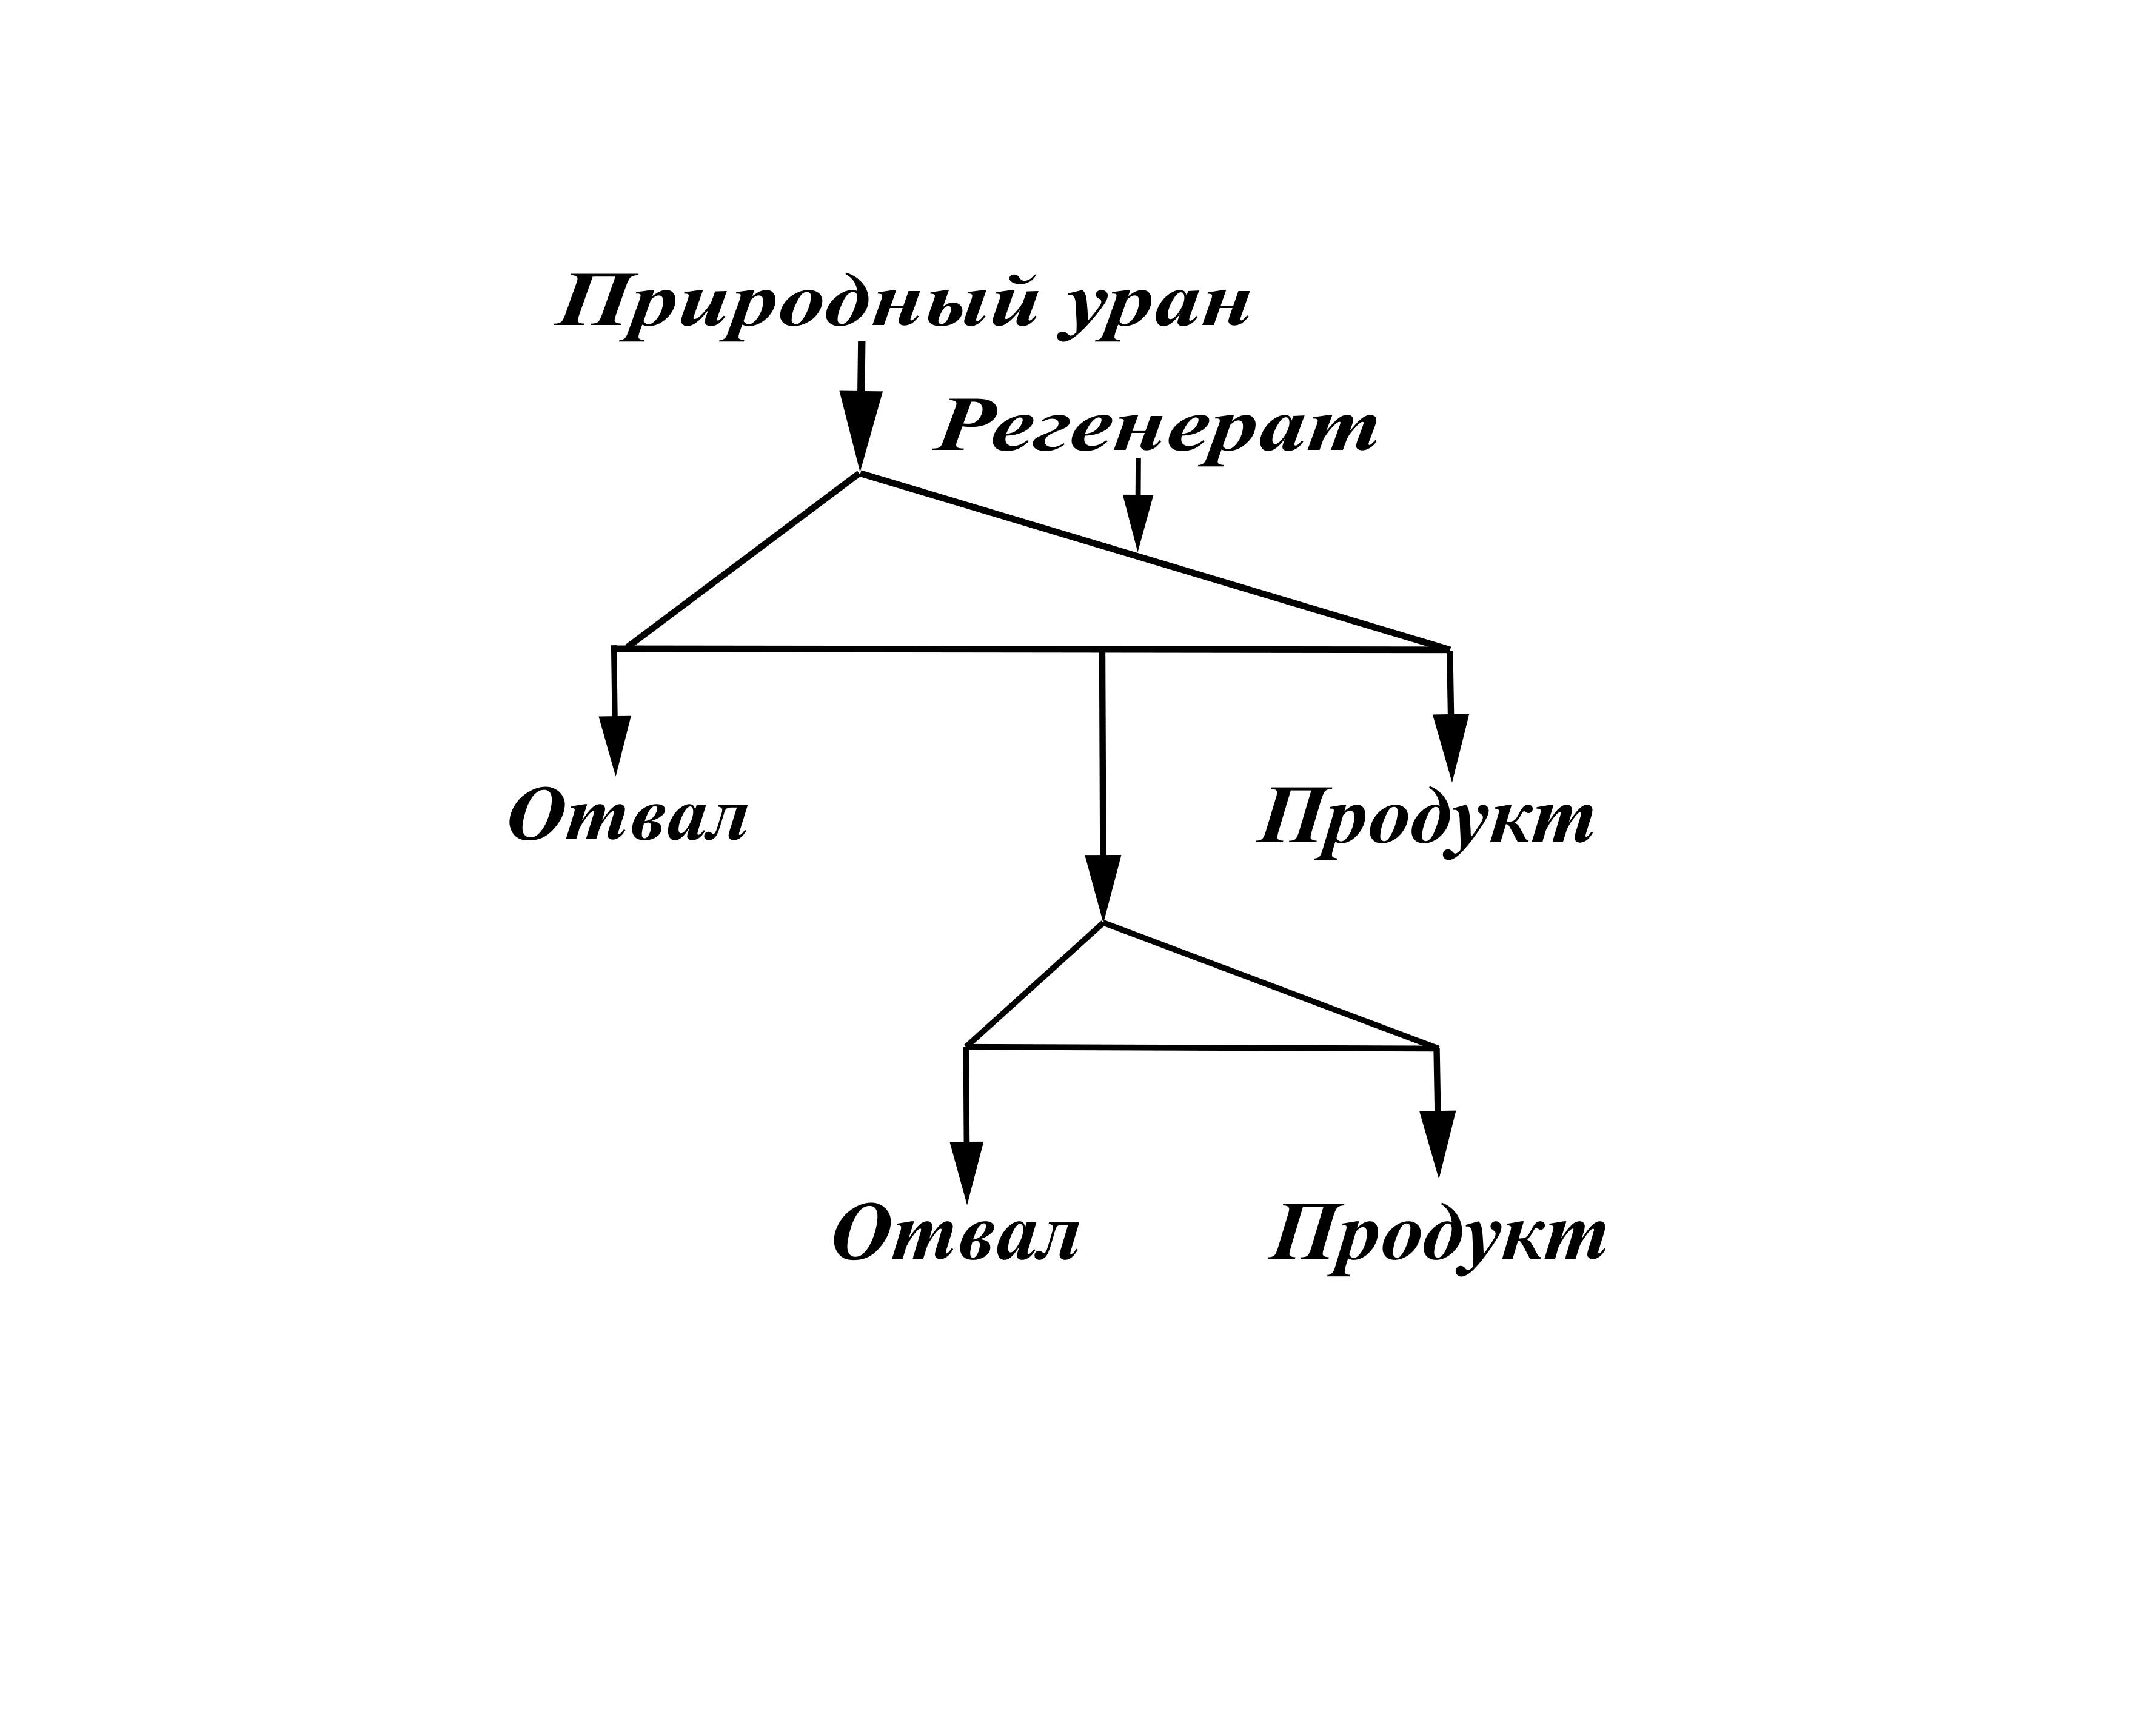
\includegraphics[scale=0.15]{cascades/int_double}}
%   \caption{Двойной каскад на основе каскада, получающего очищенный регенерат}\label{fig:int_double}
% \end{figure}

% Так как схема каскада с дополнительным потоком отбора (рис. \ref{fig:3_out}) является усовершенствованием схемы с дополнительным питанием (рис. \ref{fig:2_inputs}), продукт, получаемый в потоке <<основной отбор>> соответствует качеству товарного НОУ для легководных реакторов \cite{palkinSeparationUraniumIsotopes2010}. Однако, высокое качество очищенного регенерата достигается только при малой доле потока питающего регенерата относительно природного урана, если необходимо оставаться в рамках требований к НОУ, производимом в потоке основного отбора. Заметного снижения содержания минорных изотопов в дополнительном отборе можно добиться лишь при сильном разбавлении регенерата природным сырьем, в соотношениях, лежащих в диапазоне (1-25)/100 \cite{palkinSeparationUraniumIsotopes2010, smirnovKaskadnyeShemyZadachah2012}. 


По существу своей работы представленная на рисунке \ref{fig:3_out} каскадная схема является модификацией рассмотренной ранее схемы с двумя потоками питания. Разница состоит в наличии потока дополнительного отбора, в котором можно получить очищенный регенерат. Однако наличие этого потока накладывает определенные ограничения на соотношения между потоками природного урана и регенерата, питающих каскад. Это вызвано тем, что заметного снижения содержания минорных изотопов в дополнительном отборе можно добиться лишь при сильном разбавлении регенерата природным сырьем, в соотношениях, лежащих в диапазоне (1-25)/100 \cite{palkinSeparationUraniumIsotopes2010, smirnovKaskadnyeShemyZadachah2012}. Фактически это означает, что основной эффект «очистки» здесь обусловлен разбавлением и включением дополнительного отбора на ступени с концентрацией $^{235}$U, близкой к таковой в исходном регенерате. При этом в схеме не происходит фактического отделения $^{235}$U от четных изотопов.
Учитывая выше сказанное, каскадная схема, представленная на рисунке \ref{fig:3_out} не может обеспечить решение сформулированной выше задачи обогащения регенерата в условиях многократного рецикла по тем же причинам, по которым подобную задачу не решает прочие «разбавляющие» схемы. 
Кроме того, отдельного анализа требует вопрос дальнейшего использования получаемого в дополнительном отборе очищенного регенерированного урана. В зависимости от входящего состава обогащаемого регенерированного урана данный полупродукт может быть не пригоден для последующего прямого обогащения в ординарном каскаде и потребует хоть небольшого, но дополнительного разбавления. Это ставит вопрос о целесообразности получения такого полупродукта в принципе.




% В схеме также предусмотрена возможность значительного снижения нежелательной концентрации $^{236}$U в <<очищенном>> потоке за счет уменьшения самого этого потока.
% Этот эффект можно применить следующим образом: например, снизить концентрации $^{234}$U и  $^{236}$U в промежуточном продукте (16\% для  $^{236}$U), при этом всего лишь незначительно уменьшив (всего на 4\%) поток этого полупродукта \cite{palkinPurificationReprocessedUranium2016}. Такое понижение массового потока выходящей смеси тем более целесообразно еще и потому, что его увеличение привело бы к снижению в нем $^{235}$U. Приведенное свойство схемы, позволяющее регулировать содержание легких изотопов в дополнительном продукте, обусловлено тем, что доля массового потока, извлекаемая из потока, проходящего через промежуточную ступень каскада, определяет распределение изотопных концентраций по ступеням отборной части каскада. Так, меньшая доля изымаемого из каскада в промежуточной ступени материала, в меньшей степени препятствует концентрированию легких изотопов в основном отборном потоке каскада, а значит и снижает их концентрации в самом дополнительном отборе.

% Таким образом, схема с дополнительным отбором, по сравнению со схемой с дополнительным потоком питания (рис. \ref{fig:2_inputs}), имеет дополнительное преимущество, состоящее в извлечении из промежуточной ступени некоторого количества очищенного от нежелательных изотопов регенерата. Однако, ввиду необходимости использовать в этой схеме в несколько раз большую долю природного урана в питании, чем доля задействуемого регенерированного урана, этот каскад также является по существу схемой разбавления регенерата. В этом состоит главный недостаток схем с дополнительными потоками питания и отбора.





% Следовательно, данная схема не может обеспечить широкомасштабного возврата регенерированного урана в топливный цикл ВВЭР, ввиду малой удельной экономии природного урана.

% Таким образом, задача возврата регенерата в ЯТЦ в виде низкообогащенного урана требует дальнейших поисков эффективных схем, так как предложенный каскад рис. \ref{fig:3_out} демонстрирует снижение экономии природного урана, и не позволяет вернуть весь ОЯТ (в соотношении к продукту 1:1).

% В качестве отступления, следует заметить, что каскад с дополнительным продуктом подходит для решения задачи наработки разбавителя для ВОУ \cite{palkinPOLUChENIERAZBAVITELYaDLYa2017}, как показано в \cite{shopenSposobPolucheniyaRazbavitelya2008}, так как в качестве разбавителя необходимо использовать изотопную смесь с пониженным относительно уровня природного урана содержанием $^{234}$U, который является сильным альфа-излучателем. Использование же предварительно обогащенного обедненного урана дает возможность задействовать делящийся изотоп $^{235}$U из оружейного урана (> 90\% $^{235}$U) \cite{korotkevichRealizaciyaProgrammyVOUNOU2003,SposobPolucheniyaRazbavitelya}.

Говоря о преимуществах, свойственных рассмотренным каскадам, которые можно наблюдать из приведенного анализа схем, условно выделенных в категорию «разбавляющих». Представленные выше схемы позволяют:
\begin{enumerate}
  \item снижать концентрацию четных изотопов при обогащении регенерата различного исходного состава;
  \item	простую реализацию на основе центробежного метода разделения;
  \item в большинстве случаев, кроме схемы с разбавлением предварительно обогащенного регенерата урана (рис. \ref{fig:diagram1}.2), реализовать процесс обогащения без превышения допустимых концентраций четных изотопов на отдельных ступенях каскада.
\end{enumerate}


В качестве вывода для рассмотренных схем, необходимо обозначить следующее. Общим недостатком всех вышеупомянутых схем (рис. \ref{fig:diagram1} и \ref{fig:2_inputs}), является то, что они по существу лишь разбавляют $^{232}$U природным ураном или иным материалом, не содержащим четных изотопов $^{232,236}$U. При этом для производства на основе регенерата НОУ-продукта, приходится использовать количество <<чистого>> материала в несколько раз превышающее долю используемого регенерата, чтобы добиться снижения содержания $^{232}$U в продукте до приемлемых значений. Это обстоятельство затрудняет или делает невозможным решение сформулированной выше задачи обогащения регенерированного урана в условиях многократного рецикла урана в топливе ВВЭР. Также в качестве недостатков рассмотренных схем следует отметить, что многие из них, кроме (рис. \ref{fig:diagram1}.3), приводят к загрязнению всего используемого ими разделительного оборудования, что может затруднить последующее его использование для обогащения смесей урана, не содержащих $^{232}$U. Эти два недостатка такого рода схем стимулировали поиск подходов, позволяющих реализовать отделение $^{232}$U от изотопной смеси. Реализовать это возможно за счет появления параметров, позволяющих уменьшать относительную концентрацию изотопов $^{232}$U и $^{235}$U одновременно с обогащением последнего (и здесь и далее под относительной концентрацией компонентов понимаем отношение их абсолютных массово-долевых концентраций).

Перейдем к расмотрению возможностей преодоления недостатков рассмотренных схем, анализируя схемы использующие подход понижения относительной концентрации изотопов  $^{232}$U и $^{235}$U.

\subsection{Схемы из нескольких каскадов}

Простейшим вариантом каскада, реализующим отделение $^{232}$U от конечного продукта, является двойной каскад (рис. \ref{fig:double_ru}).
Эта модификация направлена на эффективное удаление $^{232}$U из каскада и нацелена на получение НОУ реакторного качества без необходимости вовлечения разбавителя на основе природного урана \cite{SosninYuChelcov, TehnicheskieResheniyaPo}.
Рассмотрим принципы работы такой схемы.
В простейшем варианте ее реализации, первом каскаде (верхнем) $^{235}$U обогащается вместе с легкой фракцией (отбор первого каскада на рис. \ref{fig:double_ru}), где также накапливается $^{232}$U.
Затем, эту смесь направляют во второй каскад, где самые легкие изотопы $^{232,234}$U концентрируются в загрязненной <<отборной>> части и выводятся из каскада, не попадая в конечный НОУ-продукт.
В то же время НОУ-продукт с требуемым уровнем обогащения по $^{235}$U извлекается из <<тяжелого>> (отвального) выходящего потока второго каскада. При этом в получаемом продукте контролируется соответствие требованиям по концентрациям изотопов $^{232,234}$U с одновременной компенсацией паразитного поглощения нейтронов, привносимого изотопом $^{236}$U
\begin{figure}[ht]
  \centerfloat{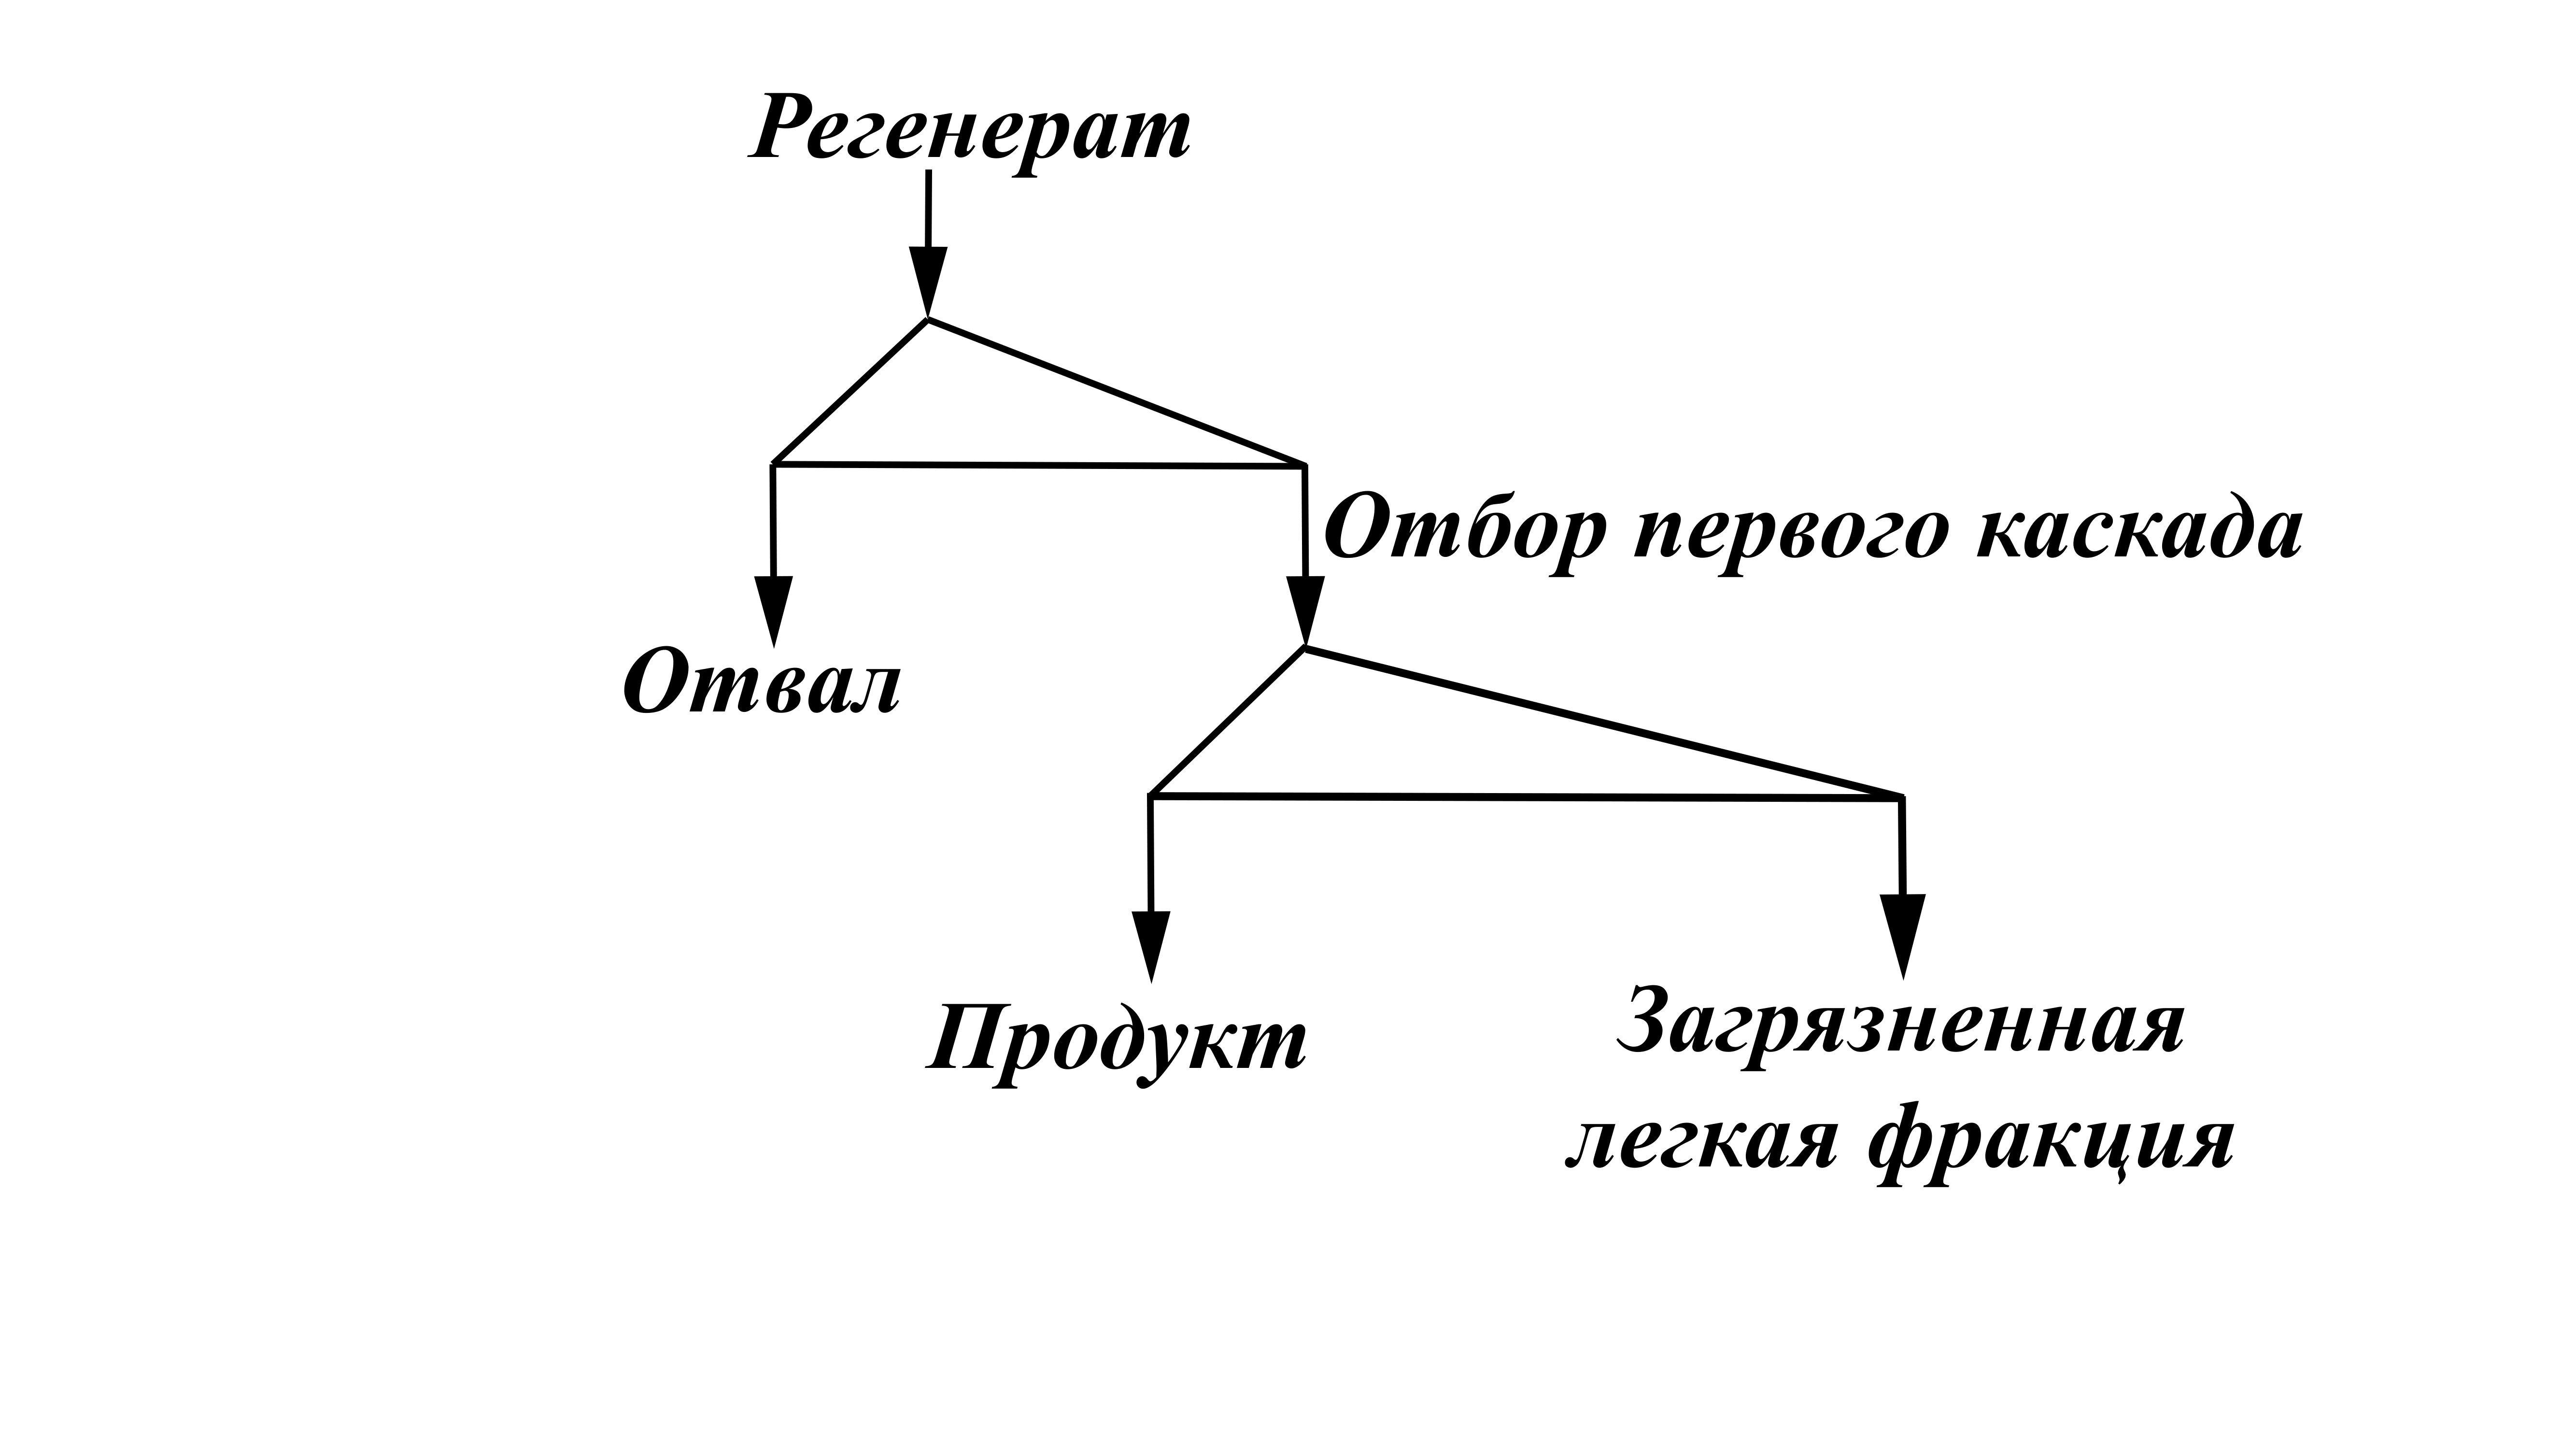
\includegraphics[scale=0.07]{cascades/double_ru}}
  \caption{Двойной каскад}\label{fig:double_ru}
\end{figure}

Эффект, который наблюдается в в выходящем потоке, сконцентрировавшем легкие изотопы, состоит в возможности сконцентрировать в этом отборе четные изотопы $^{232,234}$U, уменьшив их долю в конечном продукте. Принцип работы такой схемы состоит в следующем. Когда концентрация $^{235}$U достигает высокого уровня, соответствующего высокообогащенному урану (ВОУ),% с $^{235}$U > 20\% или близкому к этому значению,
концентрация этого изотопа достигает насыщения, при том что концентрации более легких изотопов $^{232,234}$U (а также $^{233}$U, который учитывается не во всех рассмотрениях) продолжают увеличиваться от ступени к ступени. Такая особенность массопереноса в каскаде обусловлена тем, что изотопы $^{232,233,234}$U обладают более высокими относительными коэффициентами обогащений, чем $^{235}$U \cite{borodynyaIssledovanieProblemyVovlecheniya1989}. За счет этого во втором каскаде и достигается <<пространственное>> разделение легкой фракции с изотопами $^{232,233,234,235,236}$U и тяжелой с $^{235,236,238}$U, в чем и состоит основная идея двойного каскада. В результате в получаемом товарном НОУ снижены как концентрации изотопов $^{232,234}$U, так и $^{236}$U, что крайне важно в условиях многократного рецикла урана, в котором $^{236}$U во многом определяет динамику накопления изотопа $^{232}$U в ОЯТ \cite{dudnikovInfluence236UEfficacy2016}. 

Существует также вариант реализации двойного <<очищающего>> каскада, предполагающий вывод загрязненной легкими изотопами $^{232,234}$U фракции из первого в цепочке из двух каскада \ref{fig:pure_double}. Принцип ее работы состоит в следующем.

\begin{figure}[ht]
  \centerfloat{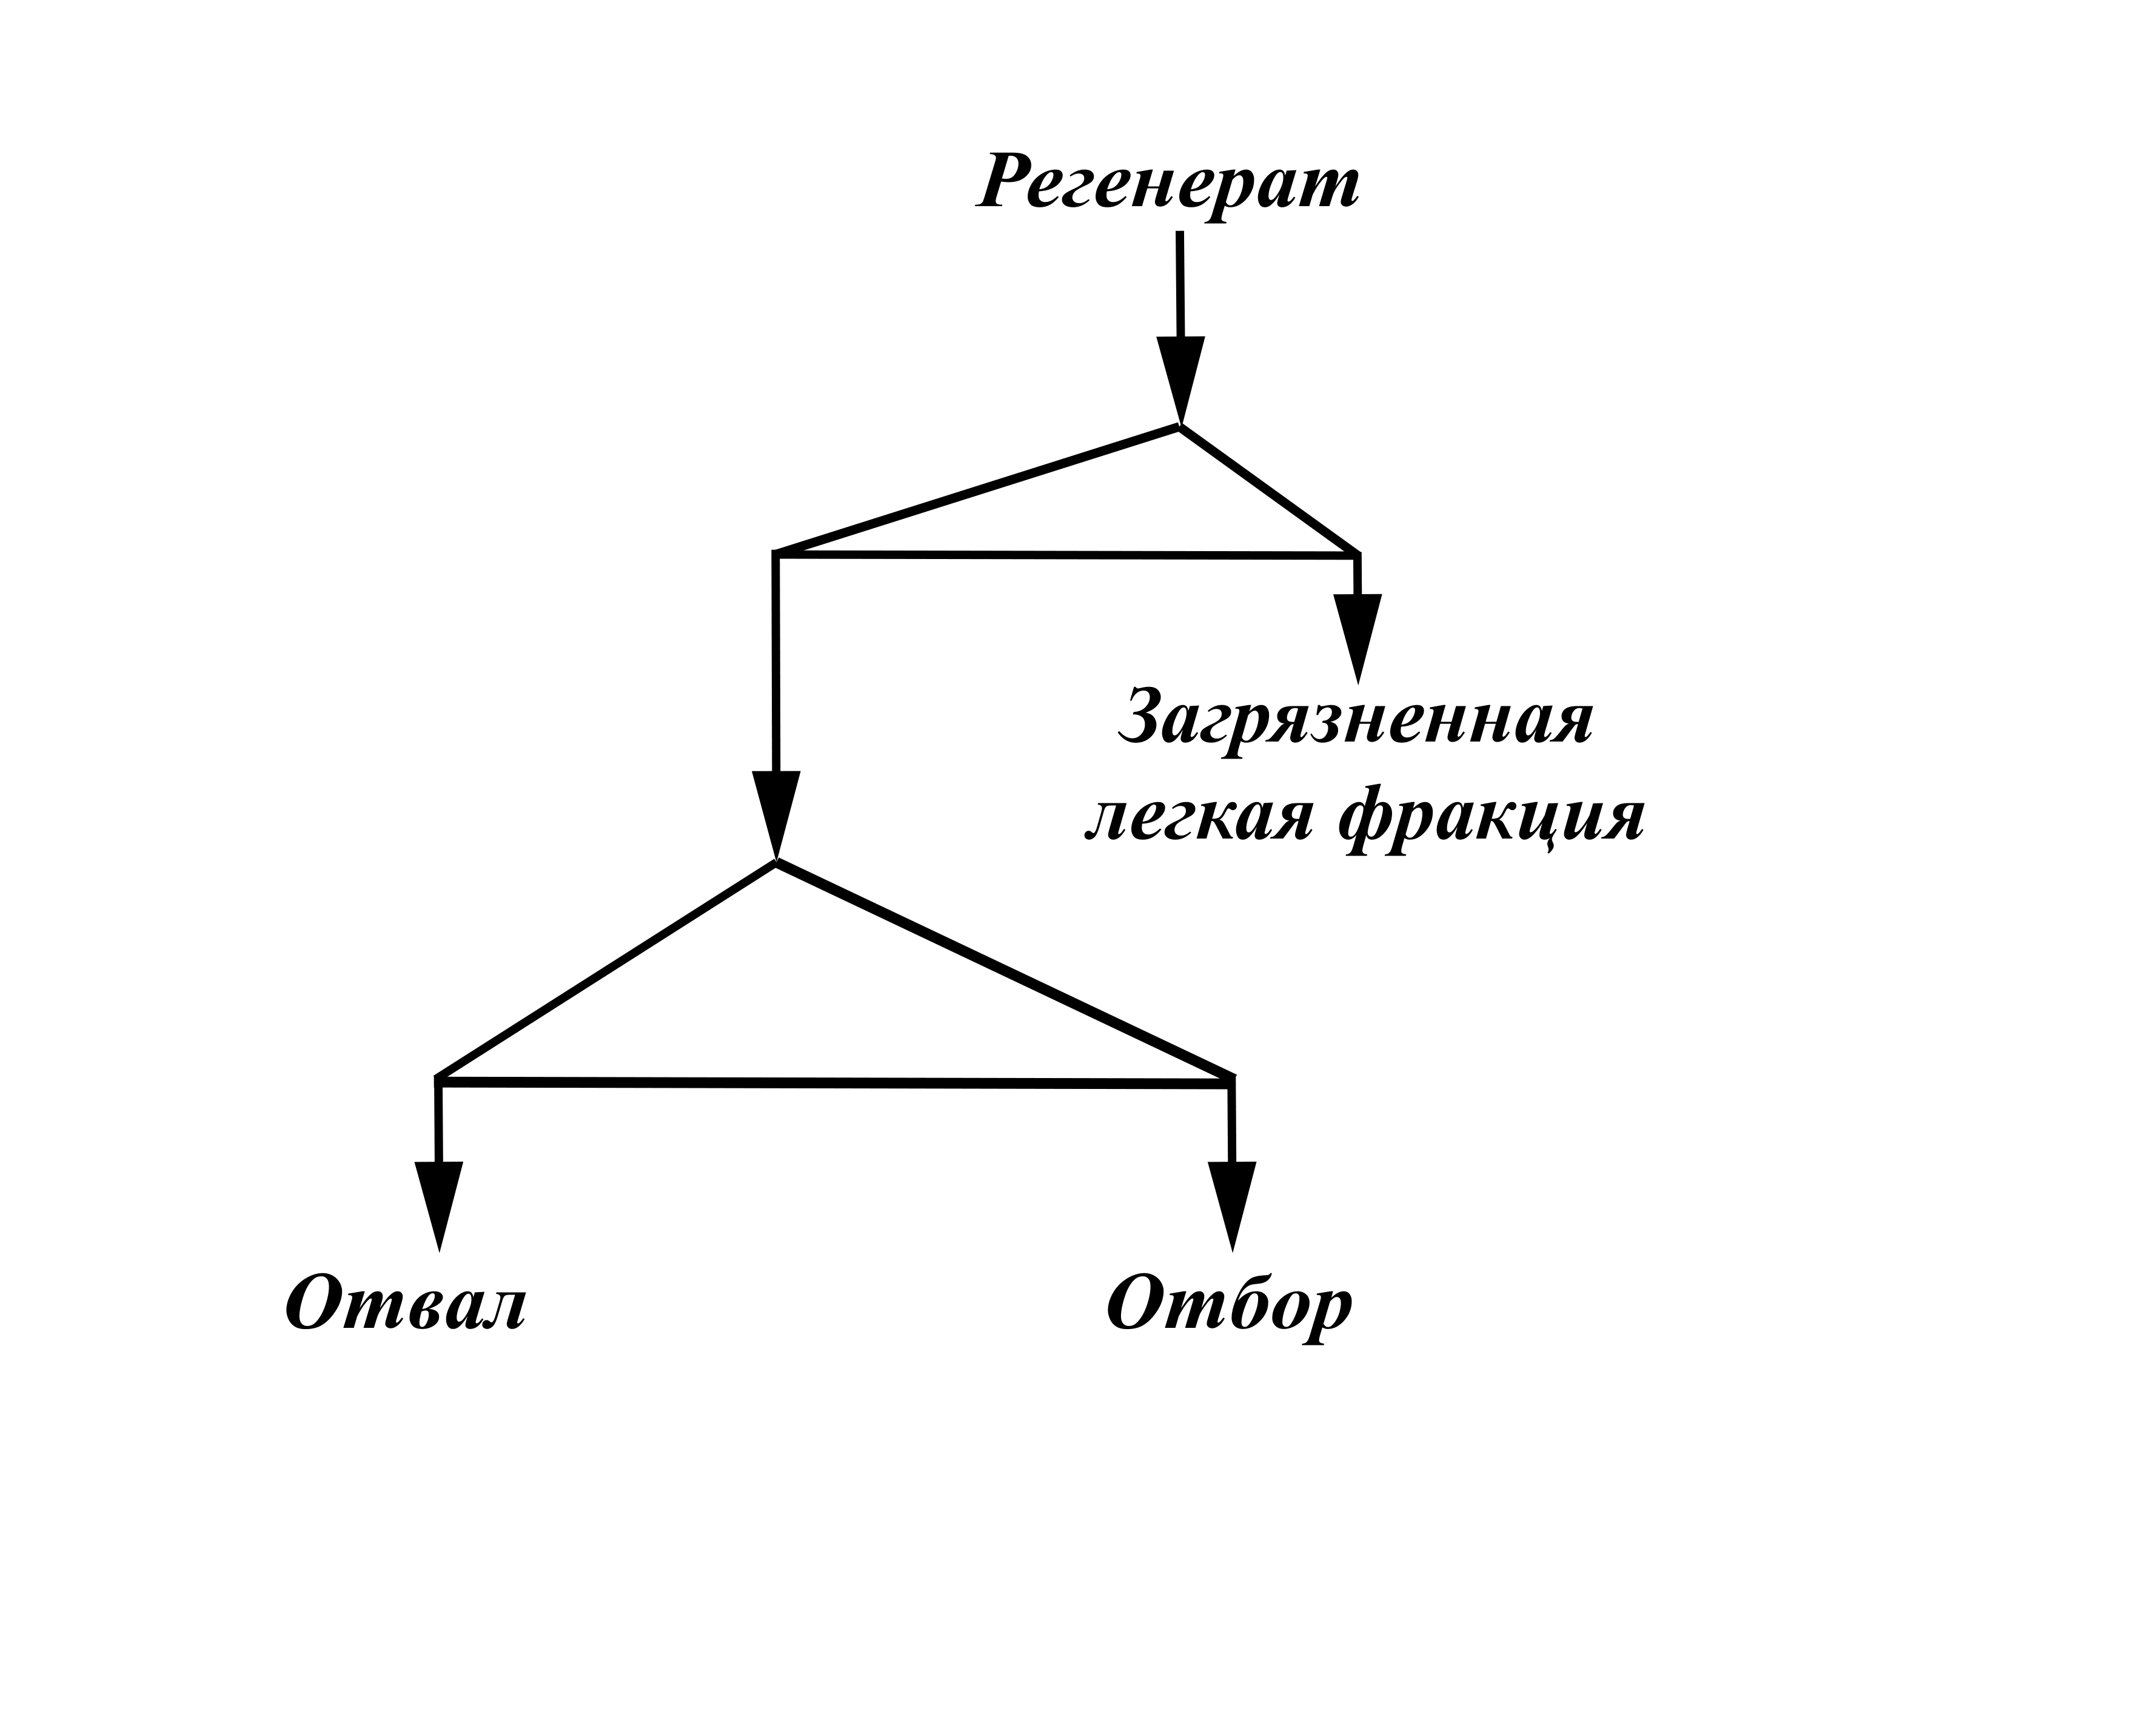
\includegraphics[scale=0.1]{cascades/pure_double}}
  \caption{Двойной каскад с очисткой в первом каскаде}\label{fig:pure_double}
\end{figure}

В первом каскаде в легкой фракции концентрируются выводимые из системы $^{232,234}$U. Затем второй каскад запитывается тяжелой фракцией первого каскада. В таком варианте схемы двойного каскада роль каскада, на котором производится очистка от легких четных изотопов, принимает первый ординарный каскад. Для такой схемы повышение степени обогащения в первом каскаде или, иными словами, удлинение обогатительной части этого каскада, позволяет добиться концентрирования большей доли $^{232,234}$U в выводимом из системы потоке, что ведет к более низкому содержанию этих изотопов в конечном продукте. В качестве примера реализации схемы двойного каскада, в патенте \cite{vodolazskihSposobIzotopnogoVosstanovleniya2006} предлагается обогащать изотопную смесь регенерата до уровня оружейного (> 90\% $^{235}$U) уже в первом ординарном каскаде. Такой подход позволяет добиваться содержания $^{232}$U в тяжелой фракции второго каскада на уровне сырьевого регенерата при рассматриваемых условиях задачи.

Как частный случай такой схемы в работе \cite{palkinOchistkaRegenerirovannogoGeksaftorida2013} предлагают использовать прием смещения точки подачи питания в сторону точки отбора легкой фракции первого каскада. Это позволяет добиться существенного снижения доли $^{232}$U в конечном продукте, поскольку прохождение ценным изотопом $^{235}$U меньшего количества последовательных ступеней каскада позволяет сохранить большую его часть в тяжелой фракции, при этом извлекая из отборной ступени легкой фракции основную часть $^{232}$U. С помощью такого подхода, можно подбирать количество ступеней каскада и расположение в нем дополнительного потока отбора, уменьшая концентрацию $^{232}$U в этом дополнительно отбираемом потоке \cite{palkinOChISTKAREGENERIROVANNOGOURANA2021}. Предварительная очистка регенерированного урана от $^{232}$U в ординарном каскаде позволяет повысить эффективность последующего его обогащения в каскаде с дополнительными потоками питания и отбора. \cite{palkinVOSSTANOVLENIEIZOTOPNOGOSOSTAVA2021}

Для обоих рассмотренных вариантов реализации двойного каскада имеют место следующие факторы.

Возможность удалять из изотопной смеси легкие четные изотопы сопряжена с потерями ценного $^{235}$U в виде высокообогащенного урана в выводимом потоке. Кроме того, так как результирующая побочная смесь содержит повышенную долю $^{232,234}$U, это обстоятельство накладывает жесткие ограничения на обращение с таким радиотоксичным материалом, поэтому возникает вопрос окончательной утилизации этого материала \cite{smirnovApplyingEnrichmentCapacities2018}.
% Таким образом, загрязненность побочно произведенной фракции легкими изотопами, и, в особенности, изотопом $^{232}$U, требует особых условий обращения с ней, а окончательная утилизация может быть крайне дорогостоящей операцией из-за того, что в таком материале превышены допустимые пределы концентрации $^{232}$U -- источника гамма-излучения \cite{smirnovApplyingEnrichmentCapacities2018}.

Увеличения эффекта очистки удается достичь при высоких концентрациях по $^{235}$U на выходе из первого каскада ($\geq$20\%) \cite{SposobIzotopnogoVosstanovleniyac}. А превышение порогового значения для ВОУ в 20\% может быть нежелательным как с точки зрения нормативных документов МАГАТЭ, согласно которым урановая смесь с концентраций $^{232}$U более 20\% считается материалом прямого использования, так и с точки зрения возникающих из-за понижения концентрации  $^{235}$U во втором каскаде потерь работы разделения \cite{ManagementHighEnriched2005}.

Эти два фактора, связанные с появлением в схеме легкой высокообогащенной фракции второго каскада, а также с высокой концентрацией $^{235}$U, достигаемой на некоторых участках схемы, наряду с отсутствием решения проблемы очистки от изотопа $^{236}$U, составляют основную проблему двойных каскадов (рис. \ref{fig:double_ru}). При этом в качестве основного достоинства понимается возможность очистки продукта от изотопов $^{232}$U и $^{234}$U, а не разбавления как в случае с ранее рассмотренными схемами.

Существуют также реализации, когда схема двойного каскада (рис. \ref{fig:double_ru}) подразумевает использование газа-носителя (или буферного газа) \cite{prusakovCorrectingIsotopicComposition2008, SposobIzotopnogoVosstanovleniyab}. Применяемое буферное газообразное соединение должно является инертным (неактивным) к гексафториду урана -- рабочему газу. Использование газа-носителя может позволить повысить эффективность отделения $^{232}$U от регенерированного урана и уменьшить потери $^{235}$U благодаря идее, которая состоит в следующем. Буферный газ с массовым числом близким к $^{232}UF_6$ подмешивается в каскадную схему с целью увеличения доли легкой фракции, отбираемой в легком потоке второго каскада, что приведет к тому, что более тяжелые изотопы, в числе которых $^{235}$U, окажутся в тяжелой фракции второго каскада. Более эффективное отделение $^{232}$U от $^{235}$U будет достигнуто за счет нарастающего объема легкой отделяемой фракции. Впервые идея применения такого газа с массовым числом, близким к $^{232}UF_6$, была выдвинута в \cite{SosninYuChelcov}, исходя из предположения, что такой газ мог бы служить матрицей-носителем для $^{232}UF_6$.
В этом исследовании авторы предложили использовать фреон-346 $C_{8}H_{3}F_{13}$, поскольку среднее массовое число этого соединения практически совпадает с массовым числом молекулы $^{232}UF_6$ (и ниже, чем у $^{235}UF_6$, что важно для предотвращения извлечения $^{235}$U в потоке газа-носителя). К тому же, $C_{8}H_{3}F_{13}$ является инертным по отношению к гексафториду урана и не вступает в реакцию с материалами газовой центрифуги. Однако такой подход накладывает ограничения на допустимый интервал давлений в разделительном процессе, который обусловлен центробежным полем газовой центрифуги \cite{prusakovCorrectingIsotopicComposition2008}.

Оба рассматриваемых варианта двойного каскада, как с газом-носителем, так и без, разделяют следующие недостатки:
\begin{enumerate}
  \item оба каскада в схеме загрязнены изотопом $^{232}$U, что осложняет радиационную обстановку на разделительном производстве;
  \item в образующейся загрязненной фракции второго каскада концентрации $^{232}$U и $^{234}$U возрастают на несколько порядков по отношению к исходной смеси, тем самым делая затруднительным обращение с подобной фракцией из-за существенного уровня удельной активности;
  \item достижение на некоторых участках схемы высокой концентрации $^{235}$U (в некоторых случаях на уровне высокообогащенного урана с содержанием $^{235}$U более 20\%), что усложняет проблему соответствия международным стандартам обращения с делящимися материалами;
  \item принципиально отсутствует возможность снижения накопления изотопа $^{236}$U, негативное влияние которого на размножающие характеристики тепловыделяющих сборок (ТВС) требует дополнительного обогащения по изотопу $^{235}$U. При этом эквивалентная концентрация $^{235}$U может быть заметно больше, чем в штатном топливе, что обуславливает дополнительные затраты работы разделения.
\end{enumerate}

При этом вариант с газом-носителем, требует очистки получаемого товарного продукта от этого газа, что, очевидно, также приводит к увеличению удельных затрат \cite{smirnovKaskadnyeShemyZadachah2012}.
% Отсюда, вариант без несущего газа более предпочтителен, поскольку в ходе технологических операций не возникает необходимости очищать от него выходную смесь \cite{smirnovKaskadnyeShemyZadachah2012}.
К тому же, имеет место следующий негативный эффект. Отделение $^{232}$U от $^{235}$U за счет использования «газа-носителя» провоцирует рост концентрации $^{236}$U в получаемом товарном НОУ. Данное обстоятельство может иметь негативные последствия в условиях многократного рецикла, поскольку рост концентраций $^{236}$U на каждом рецикле будет провоцировать рост концентрации $^{232}$U \cite{dudnikovInfluence236UEfficacy2016}.


Что касается проблемы возникновения высоких концентраций $^{235}$U, например, в \cite{palkinPurificationReprocessedUranium2016} подчеркивается, что, тогда как уже в первом же каскаде достигается концентрация $^{235}$U > 20\%, которая затем во втором каскаде еще больше повышается в потоке легкой фракции, такая схема может быть неприемлема ввиду строгих ограничений на производство ВОУ \cite{ManagementHighEnriched2005}. Для решения проблемы возникновения ВОУ, предложен вариант реализации двойного каскада, в котором исключаются высокие концентрации $^{235}$U \cite{zhurinSposobIzotopnogoVosstanovleniya2010}. В таком исполнении, принцип работы несколько меняется (рис. \ref{fig:pure_double}).

\begin{figure}[ht]
  \centerfloat{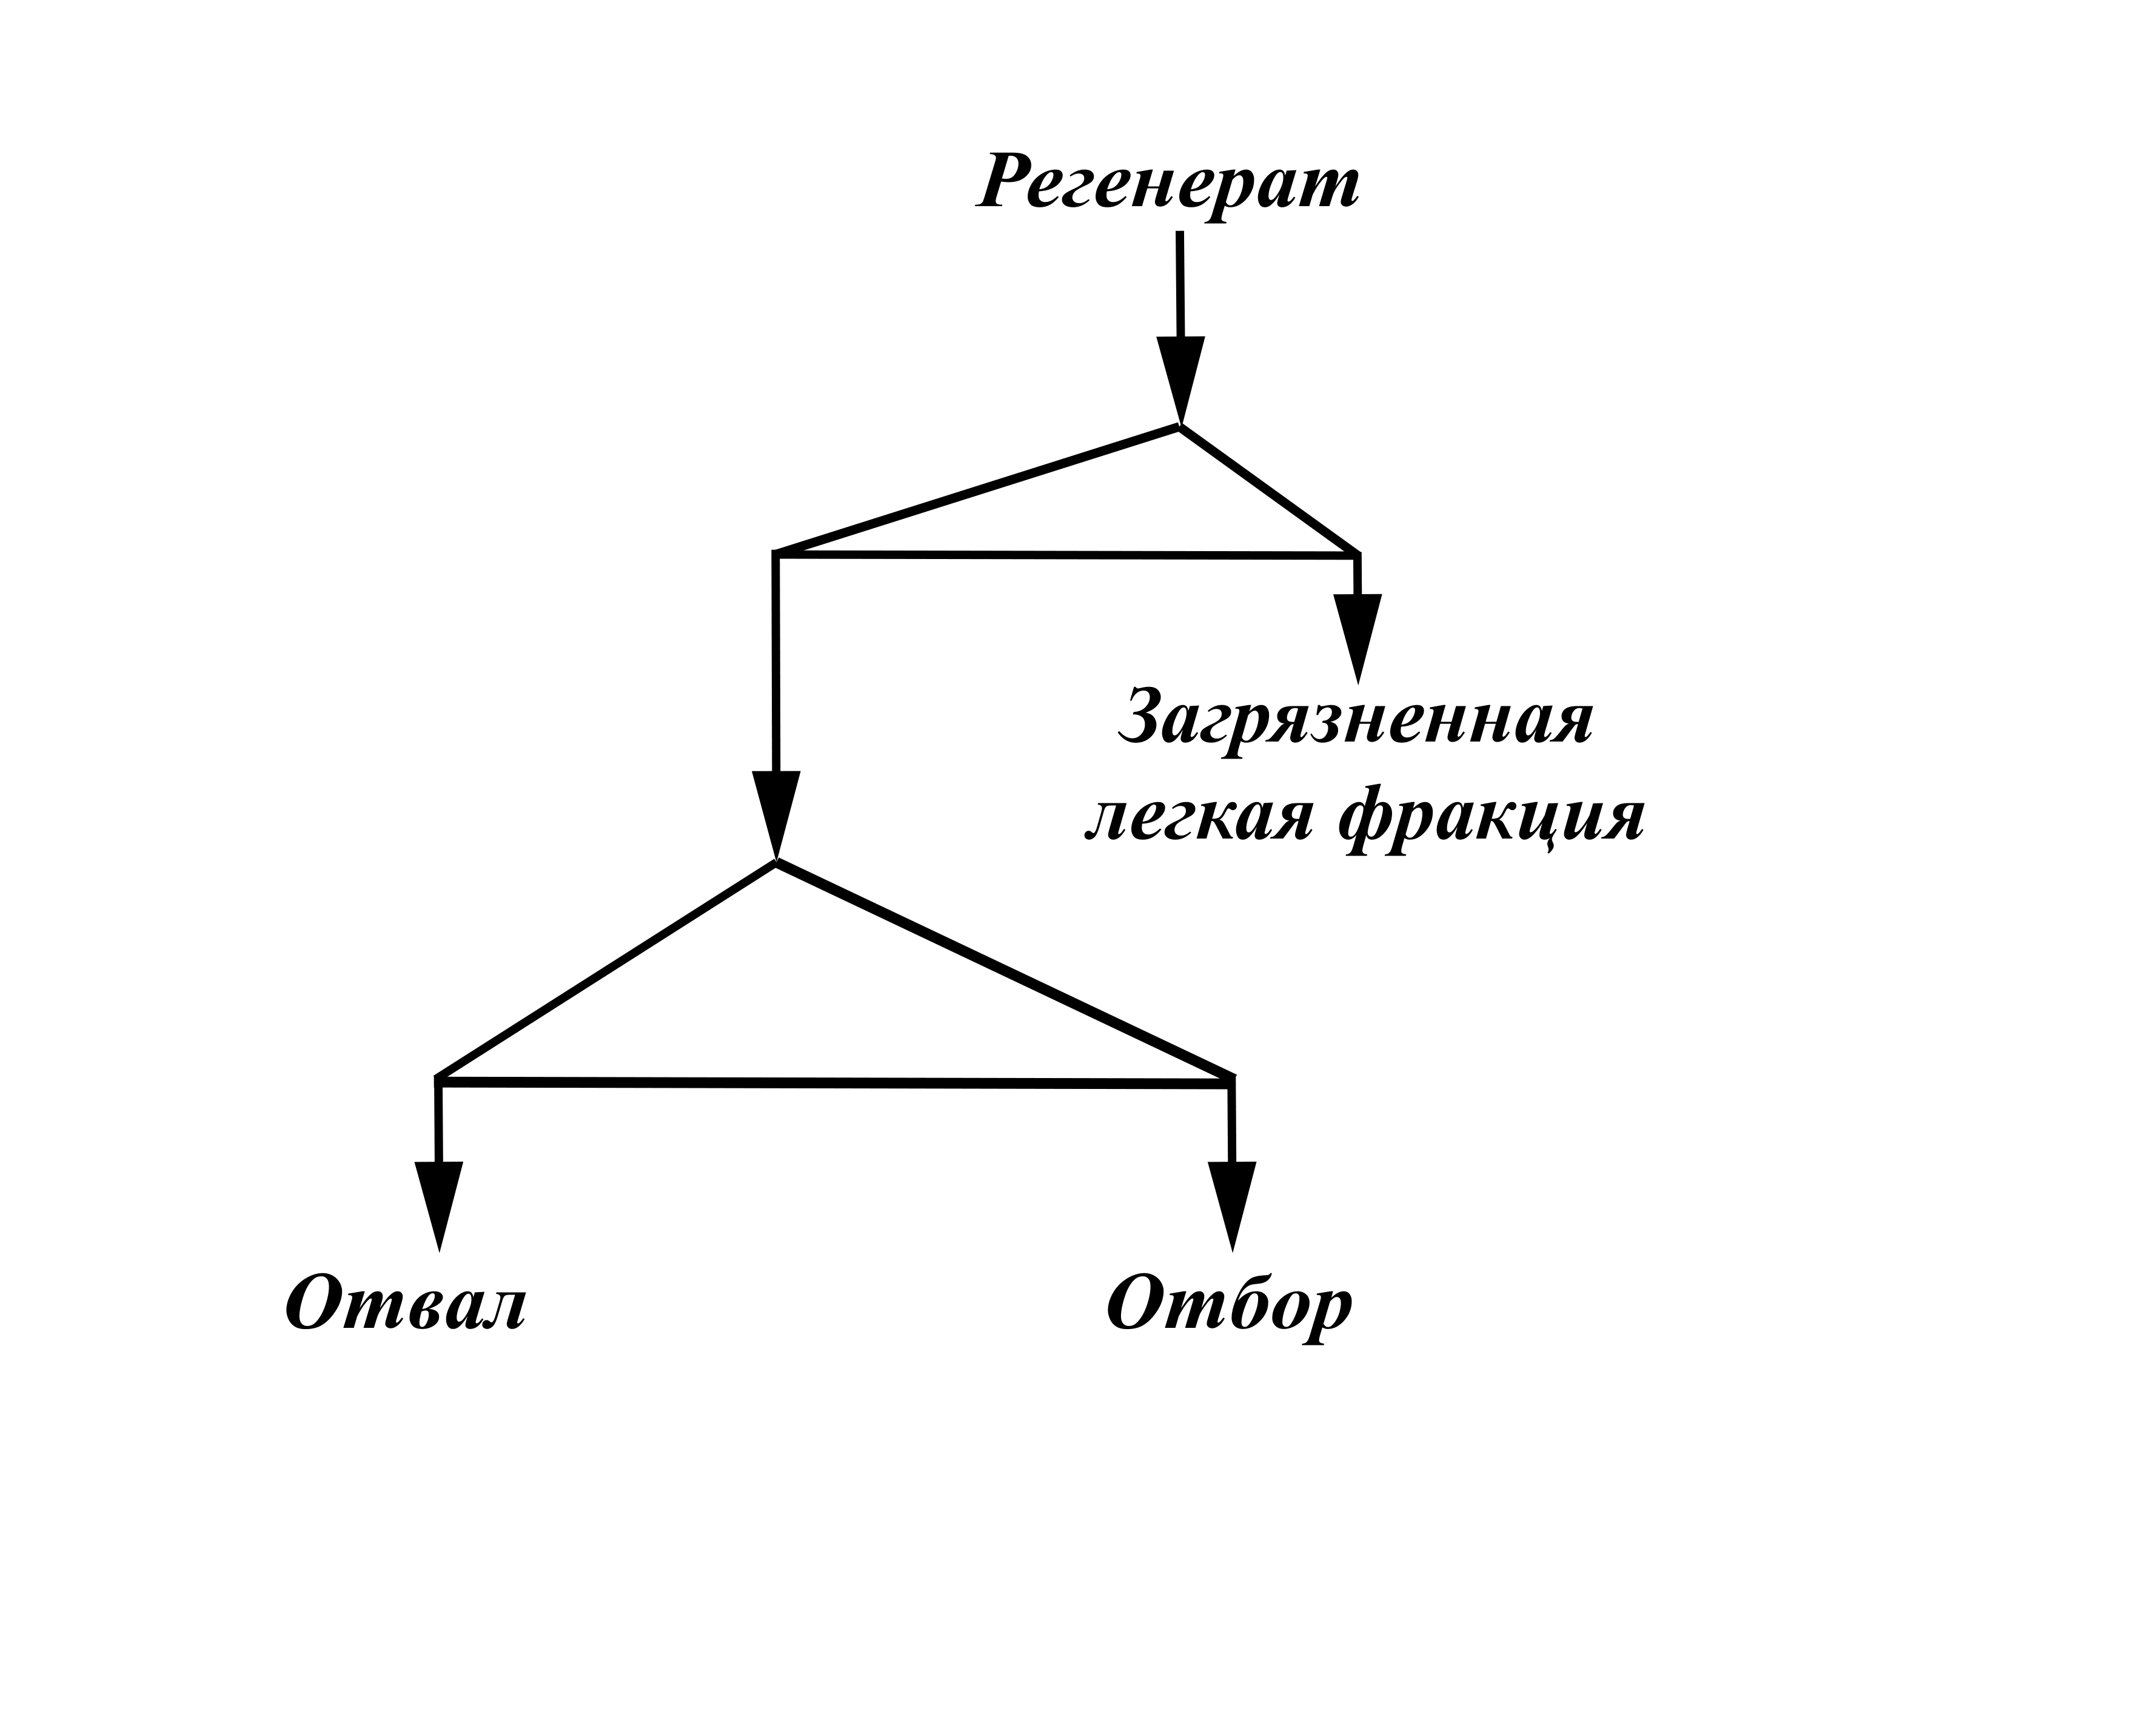
\includegraphics[scale=0.1]{cascades/pure_double}}
  \caption{Двойной каскад с очисткой в первом каскаде}\label{fig:pure_double}
\end{figure}

В этом каскаде очистка от четных изотопов $^{234,234}$U производится в первом ординарном каскаде с последующим выведением потока легкой фракции из системы. Затем, целевой продукт, восстановленный по изотопному составу, нарабатывают в легкой фракции второго каскада. Такой подход позволяет <<отсекать>> от смеси изотопы $^{234,234}$U уже в первом ординарном каскаде, передавая на второй смесь, содержащую, в основном, изотопы $^{235,236,238}$U \cite{borodynyaIssledovanieProblemyVovlecheniya1989}. А делящийся изотоп $^{235}$U, имея относительный коэффициент обогащения (относительно $^{238}$U ) выше, чем $^{236}$U, во втором каскаде будет концентрироваться в выходящем потоке легкой фракции более интенсивно.

% Возможные пути решения остальных проблем, характерных двойному каскаду предлагаются в качестве развития идеи двойного каскада.


% В главе 3 будет приведен расчетный анализ для выявления физических закономерностей, позволяющих судить о пригодности таких схем для задачи обогащения регенерата в условиях многократного рецикла.

Итак, двойной каскад позволяет повторно обогащать регенерированный уран, не разбавляя его природным ураном (или производными природного урана). Это свойство обуславливает перспективность двойного каскада для обогащения регенерата в многократном рецикле. Однако оно не предотвращает потерь $^{235}$U из топливного цикла в удаляемом потоке легкой фракции, используемой с целью вывода из системы нежелательных изотопов легкой группы $^{232,234}$U. Также использование двойного каскада не может обеспечить условие полного возврата --- возврата эквивалентного производимому продукту количества облученного материала в ядерный топливный цикл, если имеют место условия многократного использования топлива \cite{smirnovObogashchenieRegenerirovannogoUrana2018}. Это означает, что для загрузки реактора, в котором используется переработанное топливо, необходимо будет использовать другой источник делящегося изотопа $^{235}$U, например, природный уран, в отдельных тепловыделяющих элементах (ТВЭЛах) или целых ТВС, так как на основе регенерированного урана не удастся произвести количество свежего НОУ, эквивалентное массе исходного (до облучения). В результате, в контексте замыкания ЯТЦ по урановой составляющей и возврата в топливный цикл реактора всего объема топлива, реальная экономия природного урана будет далеко от 100\%.

% Чтобы решить проблему невозможности полного возврата регенерата, добившись желаемого соотношения финального продукта и питающего регенерата, потребовалась модификация схемы двойного каскада, предложенная в работе \cite{smirnovObogashchenieRegenerirovannogoUrana2018} в рамках диссертационного исследования. Она будет рассмотрена в основной части диссертационной работы (глава \ref{ch:ch3}).
% Далее продолжим детальное рассмотрение иных возможных комбинаций каскадов.

На текущий момент в теоретических работах и патентах предложен ряд модификаций двойных каскадов, появление которых было вызвано необходимостью решить задачу обогащения регенерированного урана в наиболее общей постановке. 

\subsubsection{Модификации двойных каскадов}

Одним из вариантом воплощения идеи комбинирования одиночного каскада с двумя питаниями и ординарного каскада стала схема двойного каскада, где первый каскад использует дополнительный поток питания (рис.\ref{f_2double}) \cite{palkinOchistkaRegenerirovannogoGeksaftorida2013}. Существуют два способа коммутации одиночных каскадов, при которых первым каскадом в схеме будет каскад с двумя питаниями, аналогичный каскаду, представленному на рисунке \ref{fig:2_inputs}.


\begin{figure}[ht]
  \centerfloat{\includegraphics[scale=0.5]{cascades/2double}}
  \caption{Варианты соединения двухкаскадной схемы, состоящей из каскада с двумя потоками питания и ординарного каскада: а) случай подачи отбора первого каскада на питание второго; б) случай подачи отвала второго каскада на питание второго каскада. Обозначения: $F_{nat}$ – поток природного урана; $F_{rep}$ – поток регенерата, направленного на обогащение; $P_1$ – поток «легкой» фракции каскада 1; $W_1$ – поток «тяжелой» фракции каскада 1; $P_2$ – поток «легкой» фракции каскада 2; $W_2$ – поток «тяжелой» фракции каскада 2}\label{f_2double}
\end{figure}

В рассматриваемой схеме в первом каскаде получают НОУ промежуточного обогащения, меньшего, чем требуется для получения товарного НОУ. Затем, во втором каскаде данный промежуточный материал обогащают/обедняют в одном из выходящих потоков до уровня концентрации в исходном регенерированном уране, в зависимости от того из какого потока первого каскада был получен промежуточный материал. В результате с помощью схемы на выходных потоках второго каскада производится как обогащенный товарный продукт, так и урановая смесь с концентрацией $^{235}$U на уровне исходного регенерата, но с пониженным содержанием четных изотопов. Ключевым преимуществом данной схемы, в отличие от ранее рассмотренных двухкаскадных схем, является отсутствие на каких-либо ступенях каскада концентрации $^{235}$U, превышающей уровень низкообогащенного урана.
Тем не менее, по своей сути схема является, во многом, «разбавляющей», поскольку основной эффект очистки связан с наличием в первом каскаде дополнительного питания, в котором туда поступает природный уран, выступающий в качестве разбавителя. В результате, данная каскадная схема не позволяет выполнить условие использования всего объема выделенного регенерата в условиях многократного рецикла.



Существуют и иные модификации двойного каскада, использующие в качестве одного из составных элементов каскад с двумя питаниями. Например, это может быть схема, предлагающая развитие каскада с дополнительныи потоком питания (рис.\ref{f_2double}), но использующая в качестве одного из питающих потоков регенерат не напрямую, а после предварительной очистки в ординарном каскаде \cite{palkinOchistkaRegenerirovannogoGeksaftorida2013}. Такая схема изображена на рис. \ref{fig:double_palk}, а принцип ее работы состоит в следующем.

\begin{figure}[ht]
  \centerfloat{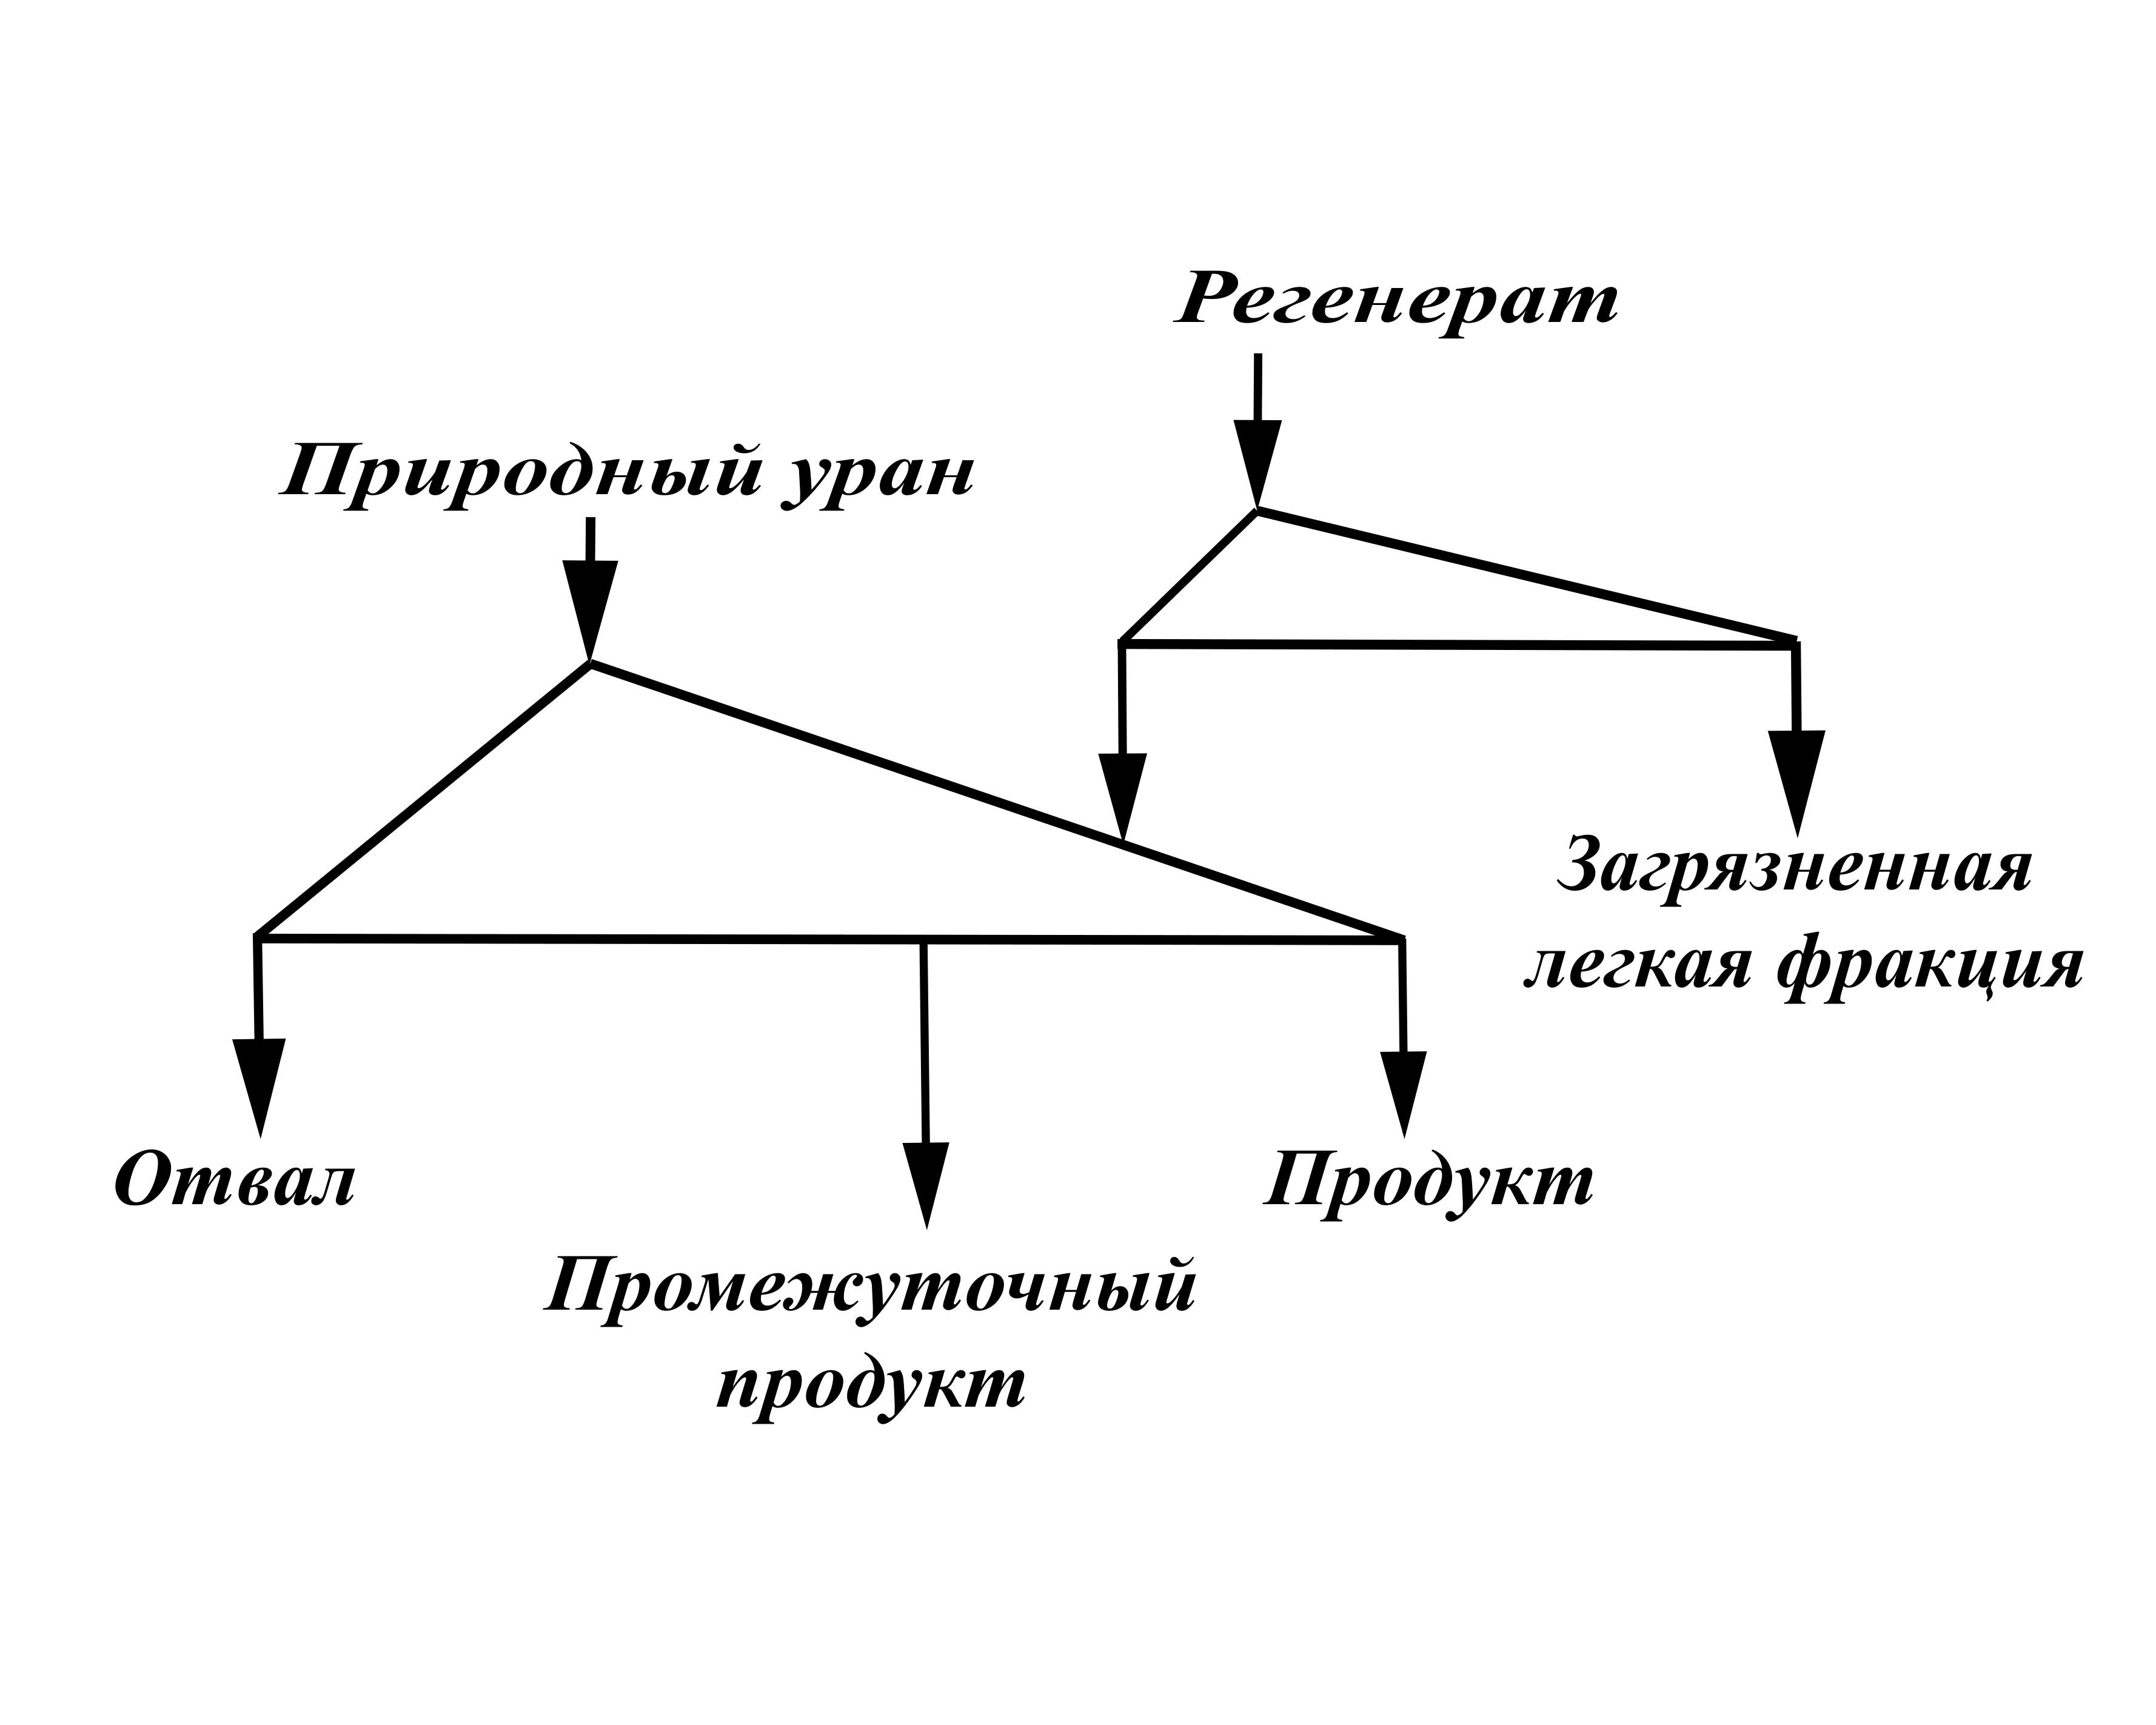
\includegraphics[scale=0.1]{cascades/double_palk}}
  \caption{Двойной каскад, использующий две стадии очистки}\label{fig:double_palk}
\end{figure}

Первый каскад, питаемый регенератом, концентрирует изотопы $^{232}$U и $^{234}$U в выходящем потоке отбора легкой фракции как в схеме двойного каскада с очисткой в первом каскаде (рис. \ref{fig:pure_double}). Полученная в другом выходящем потоке смесь тяжелой фракции первого каскада подается на промежуточную ступень второго каскада, питаемого природным ураном. Точка подачи питания этого дополнительного потока на основе очищенного регенерата подбирается по такому же принципу как и в уже рассмотренной схеме с дополнительным питанием (рис. \ref{fig:3_out}), чтобы избежать смешения потоков с различным содержанием $^{235}$U и связанных с этим потерь работы разделения. Одиночный каскад в этой схеме, питаемый природным ураном, принципиально соответствует схеме каскада с двумя питаниями и дополнительным отбором (рис. \ref{fig:3_out}), с тем отличием, что регенерированный питающий уран проходит дополнительную предварительную стадию очистки в ординарном каскаде перед поступлением в последующий каскад в качестве дополнительного питания, на которой из системы частично выводятся нежелательные четные изотопы $^{232,234}$U. При этом схема позволяет оставаться в рамках заданных ограничений, производя на выходе НОУ-продукт товарного качества и дополнительное количество промежуточного продукта с пониженным содержанием $^{232,234}$U, относительно исходного регенерата. Вдобавок, такая схема позволяет соблюсти ограничения на получение высокообогащенного урана, не выходя за 20\% по  $^{235}$U.
Дальнейшего усовершенствования схемы можно достичь с помощью оптимизации концентрации $^{232}$U в продукте, варьируя точку подачи, при этом минимизируя количество газовых центрифуг, аналогично приему, описанному для схемы двойного каскада с очисткой регенерата в первом каскаде (рис. \ref{fig:pure_double}). В этом случае, в отвале каскада будет на порядок снижено содержание $^{232}$U. Эта стадия позволяет подготовить из регенерированного урана изотопный состав с меньшим содержанием $^{232}$U для последующих этапов обогащения.

Однако такая схема имеет тот же недостаток, что и схема каскада с двумя питаниями, заключающийся в том, что высокое качество очищенного регенерата достигается только при малой доле потока питающего регенерата относительно природного урана. Иными словами, ввиду малости потока регенерата относительно потока природного урана, такая схема по свойствам ближе к схеме разбавления регенерата, чем к очищающим от $^{232,234}$U схемам. Ввиду этого, она не позволяет достичь полного возврата регенерата в цикл в условиях многократного использования ядерного топлива. Оценки приведены в приложении.


Существует еще одна модификация двойного каскада, предложенная АО «СХК», использующая в качестве одного из составных элементов каскад с двумя питаниями, одним отвалом, основным и дополнительным отбором. Такая схема предложена в патенте \cite{SposobIzotopnogoVosstanovleniyac} как возможность использовать полезные свойства каскада с дополнительным потоком питания, при этом исключая расход материала подпитки, играющего роль разбавителя регенерированного урана. Принцип такой схемы, изображенной на рис. \ref{fig:double_crazy}, состоит в следующем.

\begin{figure}[ht]
  \centerfloat{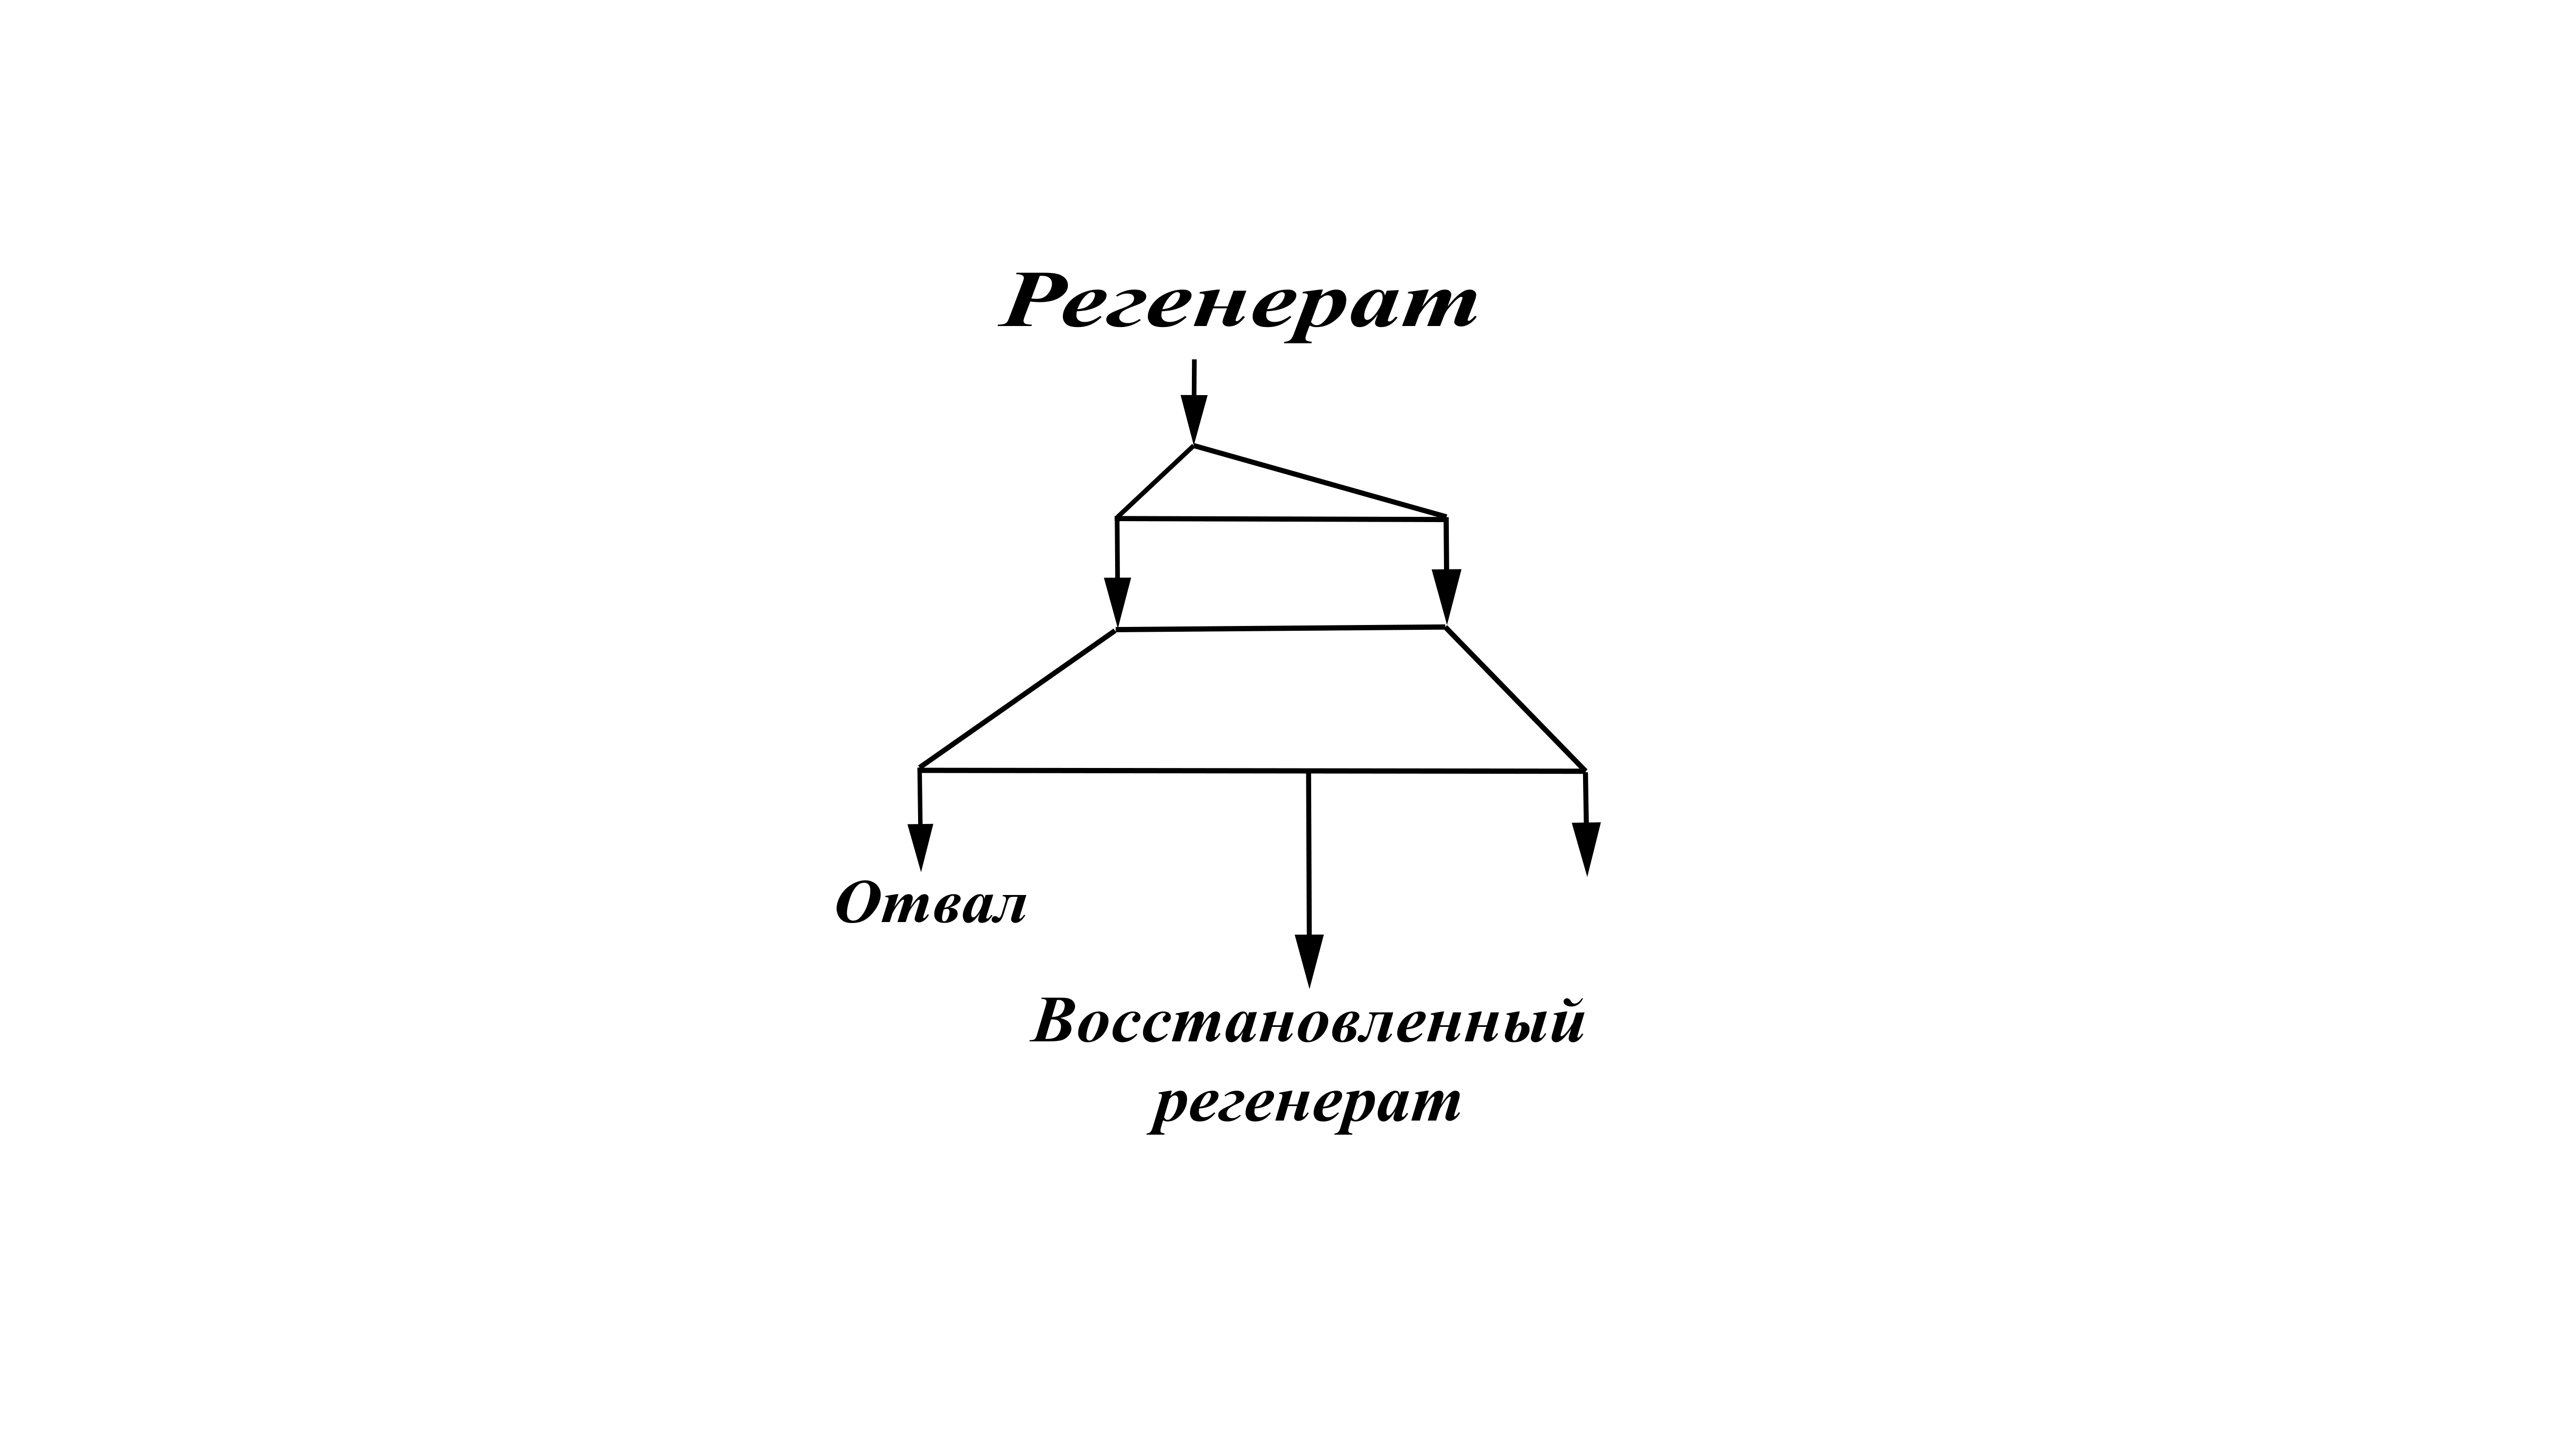
\includegraphics[scale=0.1]{cascades/double_crazy}}
  \caption{Двойной каскад на основе пятипоточного каскада, производящий восстановленный регенерат в промежуточном потоке отбора}\label{fig:double_crazy}
\end{figure}

В первом каскаде регенерированный уран обогащают изотопом $^{235}$U до $5,0-10,0$\% при поддержании соотношения массовых расходов потока отвала и потока отбора каскада в интервале (6,9–18,4) : 1. Затем, потоки отвала и отбора первого каскада подают в качестве питания на отдельные ступени второго каскада, вычисляя номера таких ступеней таким образом, чтобы концентрации $^{235}$U, которые будут установлены в ступенях каскада при его работе как можно ближе совпадали с концентрациями $^{235}$U в потоках питания. Конечный НОУ-продукт в схеме производят на одной из промежуточных разделительных ступеней центральной части второго каскада \cite{SposobIzotopnogoVosstanovleniyac}.

Рассматриваемая каскадная схема позволяет добиться разделения исходной смеси на группы, компоненты которых концентрируются в различных частях второго каскада. В результате становится возможным произвести отбор продукта из промежуточной ступени каскада, на которой концентрации изотопов $^{232,234}$U укладываются в допустимые нормативы, при требуемой концентрации целевого изотопа $^{235}$U. При этом в отличии от многих модификаций двойных каскадов в данной схеме удается избежать появления высокообогащенной фракции, что крайне важно с точки зрения вопросов обеспечения ядерного нераспространения. Тем не менее, поток легкой фракции второго каскада также имеет обогащение уровнем выше НОУ, что означает потери изотопа $^{235}$U в этом потоке. В данной схеме также удается снизить потери работы разделения по сравнению с простейшими модификациями двойных каскадов. 

Следует обратить особое внимание, что поток, произведенный в обогащающей <<легкой>> части второго каскада, имеющий категорию ВОУ, не находит своего дальнейшего применения в замыкании ядерного топливного цикла. Этот материал смешивается с отвалом второго каскада, который позволяет экранировать гамма-излучение, обусловленное $^{232}$U. Такое решение минимизирует риски долговременного хранения невостребованных продуктов изотопной корректировки регенерированного урана. То есть, это решение может быть использовано для устранения проблемы с потоком легкой фракции второго каскада схемы (рис. \ref{fig:double_ru}). Отсюда можно заключить, что основные недостатки двойных каскадов свойственны и данной схеме. 

В качестве основного вывода, касающегося схем, основанных на двойном каскаде, следует привести следующее. Такие схемы, имеют преимущество перед схемами, основанными на принципе разбавления регенерата, за счет понижения относительной концентрации изотопов  $^{232}$U и  $^{235}$U.

К ключевым же недостаткам двойных каскадных схем стоит отнести: 
\begin{enumerate}
  \item наличие отхода в виде фракции, загрязненной четными изотопами. Обращение с такой фракцией требует отработки соответствующих процедур. Важно учитывать, что традиционно обслуживание каскадов газовых центрифуг подразумевает нахождение персонала вблизи установок в процессе их эксплуатации. Наличие загрязненных изотопом $^{232}$U фракций приводит к необходимости введения дополнительных мер радиационной безопасности на производстве. В результате практическая реализации подобных мер может потребовать изменений технологических подходов, принятых на разделительных производствах;
  \item двойные каскады сами по себе принципиально не могут решить задачу «полного использования регенерата», поскольку производят продукт в количествах, в несколько раз меньших, чем требуется заданной пропорцией на единицу используемого регенерата. В связи с чем, каскадные схемы такого типа должны работать «в связке» с ординарным каскадом, обогащающим природный уран для получения топлива эквивалентного качества или иметь среди поступающих потоков дополнительный сырьевой материал, например, природный уран.
\end{enumerate}

\subsection{Каскадная схема с расширением}

Кроме описанных выше каскадов для обогащения регенерата, основанных на составных каскадах, в теоретических исследованиях предложен также вариант каскадной схемы, основанной на очистке регенерата от четных изотопов в одиночном каскаде с дополнительным потоком отбора \cite{palkinRestorationIsotopicComposition2020}. В этом подходе использован принцип выделения изотопов промежуточных массовых чисел из многокомпонентных смесей стабильных изотопов в каскадах с дополнительными потоками отбора \cite{smirnovQKASKADYDLYaPOLUChENIYa2013,smirnovVliyanieProfilyaPotoka2010,palkinMnogopotochnyeKaskadyDlya2015}. 
Основная идея работы подобной схемы состоит в том, что, подобрав соответствующим образом вид функции распределения потока питания по ступеням каскада, возможно добиться концентрирования целевого промежуточного компонента на внутренних ступенях. Организовав на ступени в области максимума концентрации целевого промежуточного компонента внутри каскада поток дополнительного отбора, возможно получить фракцию с максимальным содержанием этого изотопа при более низких по отношению к нему концентрациях легких изотопов, чем в отборе на <<конце>> каскада.
Описываемый эффект продемонстрирован как на примере модельного Q-каскада, так и на примере каскада постоянной ширины \cite{smirnovDesignCascadeLocally2015}. Каскады, имеющие подобную особенность в распределении потока питания по ступеням были названы каскадами с «расширением» потока \cite{smirnovVliyanieProfilyaPotoka2010}.
Учитывая, что изотоп $^{235}$U является промежуточным по массовому числу в смеси регенерированного урана этот способ можно применить и для концентрирования данного изотопа при обогащении регенерата урана. После чего, перемешав, полученный в промежуточном отборе такого каскада обогащенный регенерат, например, с обедненным ураном можно получить НОУ товарного качества. 
Принципиальная схема подобной каскадной установки представлена на рисунке \ref{fig:enl}.
Принцип работы данной схемы можно описать следующим образом. На вход каскада подают поток регенерированного урана $E_1$. Каскад имеет три выходящих потока: поток отвала $W_1$, поток дополнительного отбора G и поток основного отбора $P_1$. В потоке дополнительного отбора (G) достигается максимальное обогащение по $^{235}$U, которое составляет величину около 90\% или выше \cite{palkinRestorationIsotopicComposition2020}. В потоке отбора $P_1$ каскада нарабатывают смесь, высокообогащенную по $^{234}$U (до уровня 80\% и выше) и изотопу $^{232}$U (до уровня 10-3\%). Концентрация $^{235}$U в потоке $P_1$ лежит в диапазоне 10–20\%. Материал, полученный в потоке G, далее необходимо перемешать с составом, имеющим низкое содержание $^{235}$U, для получения товарного продукта с одновременным снижением концентраций четных изотопов. В качестве разбавителя удобно использовать обедненный уран (поток DepU). После смешивания потоков $E_1$ и DepU получают состав урана, обладающий необходимой для товарного продукта концентрацией $^{235}$U и удовлетворяющий ограничениям на концентрации четных изотопов.
Процесс очистки в данной схеме состоит в отделении легкой группы изотопов ($^{232}$U и $^{234}$U) от целевого $^{235}$U при одновременном снижении относительной концентрации $^{235}$U и $^{236}$U. Фактически данная схема очищает регенерат в процессе его обогащения одновременно от всех четных изотопов.

\begin{figure}[ht]
  \centerfloat{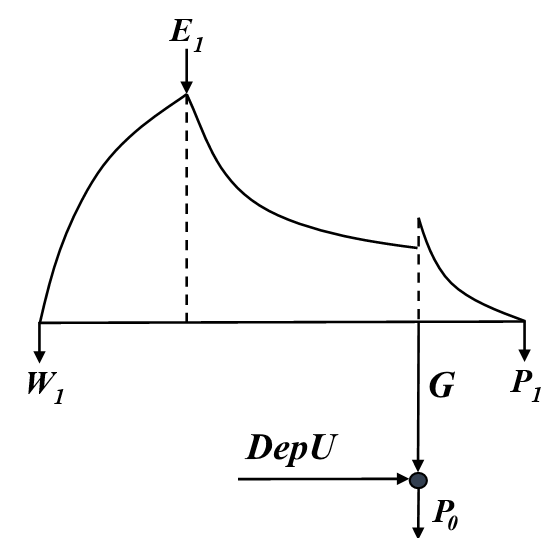
\includegraphics[scale=0.5]{cascades/enl}}
  \caption{Схема каскада концентрирования $^{235}$U в дополнительном отборе и последующим разбавлением обедненного урана для получения товарного НОУ. Обозначения: $E_1$ – поток регенерата, направленного на обогащение; $P_1$ – поток «легкой» фракции; $W_1$ – поток отвала; G – поток дополнительного отбора; DepU – поток обедненного урана; $P_0$ – поток товарного НОУ
  }\label{fig:enl}
\end{figure}


К достоинствам схемы можно отнести следующее:

\begin{enumerate}
  \item полное отсутствие природного урана в схеме и отсутствие участков обогащения обедненного урана, что экономит работу разделения;
  \item эффект коррекции изотопного состава достигается не только за счет разбавления, но и за счет снижения относительных концентрации четных изотопов к $^{235}$U (в первую очередь, $^{236}$U) в самом каскаде.
\end{enumerate}

К недостаткам схемы можно отнести следующее:
\begin{enumerate}
  \item высокие уровни активности на разделительном производстве ввиду наличия потоков с концентрациями четных изотопов на порядки, превышающими допустимые пределы для низкообогащенного урана и уранового сырья. Возможность работы разделительного производства при уровне концентрации $^{232}$U свыше 10-3\% и с фракцией, содержащей практически «чистый» $^{234}$U требует отдельной проработки с точки зрения вопросов радиационной безопасности и проблемы радиолиза рабочего вещества; 
  \item данная схема не позволяет обеспечить условие «полного использования регенерата».
\end{enumerate}


\section{Обобщенный анализ рассмотренных схем}

Подводя итог раздела, известные на сегодняшний день технические решения основаны на:
\begin{enumerate}
  \item разбавлении регенерированного урана материалами, не содержащими четных изотопов (например, природным ураном), на входе в разделительный каскад, на выходе из разделительного каскада или внутри каскада при наличии в нем двух питающих потоков (регенерат и разбавитель);
  \item получение на основе регенерата изотопной смеси с пониженным содержанием четных изотопов в каскаде с двумя питаниями и/или двумя потоками продукта (отбора);
  \item выделении из смесей регенерированного урана изотопа $^{232}$U при помощи газа-носителя, или не используя газ-носитель, в последовательном соединении двух разделительных каскадов.
\end{enumerate}

Возможности и недостатки рассмотренных схем:
\begin{itemize}
  \item основная проблема схем первого типа на основе ординарного каскада состоит в наличии в таких схемах лишь одного выходящего потока, в котором, очевидно, будут одновременно концентрироваться как целевой изотоп $^{235}$U, так и нежелательные четные изотопы. Как следствие, такого вида схемы подходят лишь для обогащения относительно незагрязненных составов регенерата, в которых исходные содержания четных изотопов меньше (на порядок или более), чем их допустимые пределы. Это означает невозможность ее применения в условиях многократного рецикла. Это ограничение связано с принципиальной невозможностью <<очищать>> изотопную смесь от четных изотопов, отделяя легкую фракцию с $^{232,233,234}$U;
  \item первые два типа схем основаны, преимущественно, на принципе разбавления изотопной смеси регенерата урана составами в которых отсутствуют изотопы $^{232,236}$U и отсутствует накапливающееся в ходе ядерных превращений дополнительное количество $^{234}$U, то есть смесями на основе природного урана. Отсутствие в них эффекта <<пространственного>> разделения изотопов легкой $^{232,233,234,235,236}$U и тяжелой $^{235,236,238}$U фракций, представляется основным недостатком таких схем, ограничивающим их применимость ввиду невозможности с их помощью достичь условия полного возврата в условиях многократного рецикла топлива. Таким образом, область их применения, если говорить о задаче возврата регенерированного урана в цикл, ограничивается работой с восстановленным ураном одного из начальных циклов переработки (первого или второго), в котором еще не накопились достаточно высокие количества $^{232}$U, чтобы сделать применение таких схем невозможным;
  \item схемы на основе двойного каскада, принцип работы которых заключается в получении результирующего НОУ-продукта на основе потока тяжелой фракции второго каскада, позволяют добиться эффективного разделения изотопов легкой $^{232,233,234,235,236}$U и тяжелой $^{235,236,238}$U фракций во втором каскаде, поэтому представляются самыми перспективными как инструмент для возврата в ЯТЦ требуемого количества ОЯТ. При дальнейшей модификации с помощью добавки к получаемому с их помощью потоку НОУ-разбавителя, можно добиться возврата регенерированного урана в топливный цикл в заданной пропорции, соответствующей полному возврату облученного топлива. На это и будет направлено дальнейшее исследование.
\end{itemize}


Таким образом, на основании проведенного анализа схем, можно заметить, что при решении задачи возврата регенерата в топливный цикл могут иметь место следующие проблемы:
\begin{enumerate}
  % \item Вывод из топливного цикла изотопов $^{232,234,236}$U можно обеспечить только посредством изотопного разделения. Концентрации этих нежелательных искусственных изотопов должны быть по-возможности уменьшены в условиях многократной переработки урановой составляющей топлива, во избежание их накопления к последующим рециклам.
  \item Предотвращение нежелательных потерь работы разделения в ходе операции разделения изотопов. Такие потери могут быть связаны с недостатками каскадных схем, когда осуществляется смешение изотопных составов с различными концентрациями $^{235}$U; 
  \item Решение вопроса с накоплением нештатных (высокотоксичных) отходов -- побочных продуктов с высокой концентрацией изотопов $^{232,234}$U.
  \item Избежание потерь $^{235}$U  в нештатных отходах c высокой концентрацией $^{235}$U, которая, в некоторых случаях, даже может превышать 20\%;
  \item Ограниченность доступных для решения задачи разделительных мощностей;
  \item Ограничения на расход дополнительного сырья (разбавителя), которым может быть как природным ураном, так и обедненным или предварительно подготовленным НОУ;
  \item Невозможность выполнения требования производства из исходного регенерата требуемого количества свежего НОУ, равного по массе исходно загруженному в реактор.
\end{enumerate}

Таким образом, рассмотренные каскады, как показывают оценки, ограничены в возможности применения для задействования всего облученного урана в заданной пропорции к производимому свежему топливу, и требуют дальнейших модификаций, которые и будут предложены в основной части диссертационной работы. 
